\documentclass[aspectratio=169,pdftex,dvipsnames]{beamer}
\usetheme[right,hideallsubsections]{Berkeley}
\usecolortheme{seahorse}
\beamertemplatenavigationsymbolsempty 
\addtobeamertemplate{footnote}{\hskip -2em}{}


\usepackage{caption}
\captionsetup[figure]{labelformat=empty,font=small}

%packages and definitions
\usepackage{wrapfig}
\usepackage{textgreek}
\usepackage{enumitem}
\setlist[itemize]{label=\textbullet}
\usepackage{amsmath,cancel,nicefrac}
\usepackage{ulem}
\usepackage{graphicx,animate}
\graphicspath{{./img/},{}} %path to graphics
\usepackage[yyyymmdd]{datetime} %date format
\renewcommand{\dateseparator}{.}

%%%%%
\usepackage{pgf,pgfplots}
\usepackage{tikz,grffile} % required for drawing custom shapes
\usetikzlibrary{shapes,arrows,automata,trees}
\pgfplotsset{compat=newest}
%\usepgfplotslibrary{patchplots}
%%%%%

\usepackage{booktabs} % nice rules (thick lines) for tables
\usepackage{microtype} % improves typography for PDF
\usepackage{verbatim}

\usepackage[acronym,nomain,nonumberlist]{glossaries}
%\makenoidxglossaries

\usepackage{xcolor,colortbl} %change font color
\usepackage[numbers,sort&compress]{natbib} %use 'numbers' for numbered citations; 'round' for () instead [] for inline citations; nsf.bst
\usepackage{bibentry}
\usepackage[eulergreek]{sansmath}


\setlength{\bibsep}{0pt} %sets space between references
%\renewcommand{\bibsection}{} %suppresses large 'references' heading
\renewcommand\bibpreamble{\vspace{-0.2\baselineskip}} %sets spacing after heading if not using default references heading

%%%%% user commands
\newcommand\blfootnote[1]{%
  \begingroup
  \renewcommand\thefootnote{}\footnote{#1}%
  \addtocounter{footnote}{-1}%
  \endgroup
}

%Fix centering on title slide which doesn't have a sidebar [plain]
\newcommand\noside{\addtolength\textwidth{2cm} 
\setlength\hsize{\textwidth} 
\setlength\columnwidth{\textwidth}
\vfill\centering}

%Make sidebar background color so it appears invisible
\newcommand\outlineframe{
    \setbeamercolor{sidebar}{fg=Chrome,bg=Chrome}
\setbeamercolor{title in sidebar}{fg=Chrome}
\setbeamercolor{author in sidebar}{fg=Chrome}
\setbeamercolor{section in sidebar}{fg=Chrome}
}

%Make sidebar original color so it appears again
\newcommand\stopoutlineframe{
    \setbeamercolor*{sidebar}{fg=PrideGold,bg=Black}
\setbeamercolor*{title in sidebar}{fg=PrideGold}
\setbeamercolor*{author in sidebar}{fg=PrideGold}
\setbeamercolor*{section in sidebar}{fg=PrideGold}
}

\makeatletter
\setlength{\beamer@headheight}{1cm}
\renewcommand{\@biblabel}[1]{#1.\hfill} %bibliography ordered list has numbers left flush
\makeatother
\setbeamertemplate{navigation symbols}{}
% \setbeamertemplate{footline}[frame number]
\setbeamertemplate{sidebar right}[sidebar theme]
\addtobeamertemplate{sidebar right}{}{%
    \vspace{10pt}
    \hspace{20pt}
    \insertframenumber
    \vspace{10pt}
    }

% Current section in TOC
\AtBeginSection[ ]
{\outlineframe
\begin{frame}{}
    \tableofcontents[currentsection,hideothersubsections]
\end{frame}
\stopoutlineframe}

 \AtBeginSubsection[]{
     \begin{frame}{}
         \vfill
         \centering
         \begin{beamercolorbox}[sep=8pt,center,shadow=true,rounded=true]{title}
             \usebeamerfont{title}\insertsubsectionhead\par
         \end{beamercolorbox}
       
         \vfill
       
     \end{frame}
 }

\logo{
\includegraphics[width=40pt]{logocorner}}

% colors
\definecolor{PrideGold}{RGB}{241,179,0}
\definecolor{Silver}{RGB}{165,169,180}
\definecolor{White}{RGB}{255,255,255}
\definecolor{Black}{RGB}{25,25,25}
\definecolor{Chrome}{RGB}{245,245,245}

\setbeamercolor{background canvas}{bg=Chrome}
\setbeamercolor{block title}{bg=Silver,fg=Black}
\setbeamercolor{block body}{bg=Silver!20,fg=Black}

\setbeamercolor{block title alerted}{bg=Black, fg=Silver}
\setbeamercolor{block body alerted}{bg=PrideGold, fg=Black}
\setbeamercolor{alerted text}{fg=Silver}

\setbeamercolor*{block title example}{bg=PrideGold, fg = Black}
\setbeamercolor*{block body example}{bg=PrideGold!20, fg = Black}

\setbeamercolor*{palette primary}{bg = PrideGold}
\setbeamercolor*{palette secondary}{bg = PrideGold, fg = White}
\setbeamercolor*{palette tertiary}{bg = PrideGold, fg = White}
\setbeamercolor*{titlelike}{fg = PrideGold}
\setbeamercolor*{title}{bg = Black, fg = PrideGold}
\setbeamercolor*{item}{fg = PrideGold}
\setbeamercolor*{caption name}{fg = PrideGold}

\setbeamercolor*{sidebar}{fg=PrideGold,bg=Black}
\setbeamercolor*{title in sidebar}{fg=PrideGold}
\setbeamercolor*{author in sidebar}{fg=PrideGold}
\setbeamercolor*{section in sidebar}{fg=PrideGold}


\setbeamercolor{section in toc}{fg=Black}
\setbeamercolor{subsection in toc}{fg=Black}

\setbeamercolor{page number in head/foot}{fg=Silver,bg=Black}
\setbeamercolor{footline}{bg=Black}

\setbeamercolor{bibliography entry author}{fg=Black}
\setbeamercolor{bibliography entry note}{fg=Black}
\setbeamercolor{bibliography entry title}{fg=Black}

% Font Information

\usefonttheme{professionalfonts}

\setbeamerfont{title}{size=\large}
\setbeamerfont{subtitle}{size=\small}
\setbeamerfont{author}{size=\small}
\setbeamerfont{date}{size=\small}
\setbeamerfont{institute}{size=\small}
\setbeamerfont{caption}{size=\tiny}

\newcommand{\edit}[1]{\textcolor{blue}{#1}} %shortcut for changing font color on revised text
\newcommand{\fn}[1]{\footnote{#1}} %shortcut for footnote tag
\newcommand*\sq{\mathbin{\vcenter{\hbox{\rule{.3ex}{.3ex}}}}} %makes a small square as a separator $\sq$
\newcommand{\sk}[1]{\sout{#1}} %shortcut for strike-through
\newcommand{\x}{\cellcolor{lightgray}\textbf{X}} %use to shade in table cell

%fix spacing for frames with subtitles
\newcommand\cST{\vspace{-0.5cm}} %Center title when no subtitle
\newcommand\ST{\vspace{-0.15cm}}  %Make subtitles fix in top bar

\newcommand{\acf}{\acrfull} %full acronym
\newcommand{\acl}{\acrlong} %long acronym
\newcommand{\acs}{\acrshort} %short acronym
\newcommand{\acfp}{\acrfullpl} %full acronym plural
\newcommand{\aclp}{\acrlongpl} %long acronym plural
\newcommand{\acsp}{\acrshortpl} %short acronym plural
\newcommand{\Acf}{\Acrfull} %full acronym first letter capital
\newcommand{\Acl}{\Acrlong} %long acronym first letter capital

\newacronym{pid}{PID}{Proportional-Integral-Derivative}
\newacronym{npp}{NPP}{Nuclear Power Plant}
\newacronym{msnb}{MSNB}{Molten Salt Nuclear Battery}
\newacronym{msr}{MSR}{Molten Salt Reactor}
\newacronym{msre}{MSRE}{Molten Salt Reactor Experiment}
\newacronym{lwr}{LWR}{Light Water Reactor}
\newacronym{smr}{SMR}{Small Modular Reactor}
\newacronym{nrc}{NRC}{Nuclear Regulatory Commission}
\newacronym{ans}{ANS}{American Nuclear Society}
\newacronym{inl}{INL}{Idaho National Laboratory}
\newacronym{nrel}{NREL}{National Renewable Energy Laboratory}
\newacronym{oak}{ORNL}{Oak Ridge National Laboratory}
\newacronym{lti}{LTI}{Linear Time-Invariant}
\newacronym{mm}{MIMO}{Multi-Input Multi-Output}
\newacronym{ss}{SISO}{Single-Input Single-Output}

\newcommand{\UF}[1][4]{$UF_{#1}$}
\newcommand{\flinak}{$FLiNaK$ }

\newcommand{\B}[1][]{$^{#1}B$ }
\newcommand{\Be}[1][]{$^{#1}Be$ }
\newcommand{\I}[1][135]{$^{#1}I$ }
\newcommand{\Xe}[1][135]{$^{#1}Xe$ }
\newcommand{\Nd}[1][149]{$^{#1}Nd$}
\newcommand{\Pm}[1][149]{$^{#1}Pm$ }
\newcommand{\Sa}[1][149]{$^{#1}Sa$ }
\newcommand{\Gd}[1][157]{$^{#1}Gd$ }
\newcommand{\U}[1][]{$^{#1}U$ }
\newcommand{\Pu}[1][239]{$^{#1}Pu$ }
\newcommand{\Ca}[1][]{$^{#1}Ca$ }
\newcommand{\Am}[1][]{$^{#1}Am$ }
\newcommand{\Po}[1][]{$^{#1}Po$ }
\newcommand{\Ra}[1][]{$^{#1}Ra$ }
%%%%%
\newcommand{\sci}[1][]{$\times$ 10\textsuperscript{#1} }
%%%%%

\title[MSNB Modeling \& Control]{Dynamic System Modeling \& PID Controller Design \\for a Molten Salt Microreactor}
\author{Sam J. Root}
\institute[Idaho Falls Center]{University of Idaho $\sq$ Idaho Falls Center for Higher Education\\
    Department of Nuclear Engineering and Industrial Management\\
    }

\date{December 6\textsuperscript{th}, 2023}    

\titlegraphic{
\includegraphics[width=0.20\textwidth]{logo}}

\begin{document}
    \nobibliography*
{    \setbeamertemplate{footline}{} 
    \begin{frame}[plain]{}
        \noside
        \titlepage
    \end{frame}
} 

\begin{frame}{About the Author}
    \vfill
    \begin{block}{Experience}
      B.S Chemical Engineering (2015-2019) - Michigan Technological University\\
      M.S. Nuclear Engineering (2021-2023) - University of Idaho - \acs{nrc} Fellow\\
      Modeling and Simulation Intern at Idaho National Lab
    \end{block}
    \vfill
    \begin{block}{Select Publications}
    \bibentry{RootXe}\;\\
    \bibentry{RootWSC}   
    \end{block}
    \vfill
\end{frame}

{\outlineframe
\begin{frame}{Outline}
    \tableofcontents[hideallsubsections]
\end{frame}
\stopoutlineframe}

\section{The Molten Salt Nuclear Battery}
\begin{frame}{Background}
    \begin{block}{Gen-IV}
        \only<1>{
            \begin{itemize}
                \item Complete re-designs
                \item Smaller footprint
                \item Deployability
                \item Versatility
            \end{itemize}
        }
    \end{block}
    
    \begin{block}{Molten Salt Reactors}
        \only<2>{
            \begin{itemize}
                \item High temperature
                \item Low pressure
                \item High specific heat
            \end{itemize}
        }
    \end{block}
    
    \begin{block}{Microreactors}
        \only<3>{
            \begin{itemize}
                \item Less than 50 MW
                \item Assembly line manufacturing
                \item Deliver/installation vs. construction
            \end{itemize}
        }
    \end{block}
\end{frame}

\begin{frame}{Molten Salt Nuclear Battery}
    \begin{columns}
        %Column 1
        \begin{column}{0.5\textwidth}
            \begin{block}{Fuel/Primary Coolant}
                \only<1>{
                    \begin{itemize}
                        \item Self-Contained liquid fueled molten salt micro-reactor 
                        \item 10 year design
                        \item 10 MWth using HALEU \UF \; dissolved in \flinak
                        \item Natural circulation driven
                    \end{itemize}
                }
            \end{block}
            \begin{block}{Control Drums}
                \only<2>{
                    \begin{itemize}
                        \item Criticality is manipulated using axial control drums 
                        \item Neutron absorber plate covering cylinders of neutron reflector
                        \item Drums are rotated to point more absorber towards the core to insert negative control reactivity
                    \end{itemize}
                }
            \end{block}
            
                
                
                
        \end{column}
        %Column 2
        \begin{column}{0.5\textwidth}
            \only<1>{
            \begin{figure}[!ht]
                \centering
                \begin{tikzpicture}
    %Core
    \draw node at (1.5,1.5) {Core};
    \draw[red, very thick] (0,0) rectangle (3,3);
    \filldraw[red,opacity=0.2] (0,0) rectangle (3,3) ;
    %Riser/Chimney
    \draw[->] (1.5,3) -- (1.5,3.5);
    %HEX
    \draw node at (1.5,4) {Heat Exchanger};
    \draw[blue, very thick] (0,3.5) rectangle (3,4.5);
    \filldraw[blue,opacity=0.2] (0,3.5) rectangle (3,4.5) ;
    %Downcomer
    \draw[->] (3,4) -- (3.5,4) -- (3.5,-0.5)  -- (1.5,-0.5);
    \draw[->] (0,4) -- (-0.5,4) -- (-0.5,-0.5)  -- (1.5,-0.5);
    \draw[->] (1.5,-0.5) -- (1.5,0);
\end{tikzpicture}

                \caption{Simplified schematic drawing of an \acs{msnb}}
                \label{fig:tikz_msnb}
            \end{figure}
            }
            \only<2>{
                \begin{figure}
                    %\animategraphics[width=0.8\textwidth, controls, loop, trim=12cm 1.5cm 2cm 2.5cm]{1}{./img/Plotter/drum/XY-}{0}{2}+
                    \resizebox*{\textwidth}{!}{\begin{tikzpicture}
    \definecolor{BGreen}{rgb} {0.143,0.5,0.237}
    \definecolor{FGreen}{rgb} {0.243,0.7,0.337}
    %Reflector
    \draw[blue, very thick] (0,0) circle (3);
    \draw[blue, very thick] (0,0) circle (1.05);
    \filldraw[blue,opacity=0.2, even odd rule] (0,0) circle (3) circle (1);
    \draw node at (4,2) {Reflector};
    \draw[->] (3.9,1.8) -- (2.5,1);
    \draw node at (-4,-2) {Control Drum};
    \draw[->] (-3.9,-1.8) -- (-2,0);
    %Core
    \draw[red, very thick] (0,0) circle (1);
    \filldraw[red,opacity=0.2] (0,0) circlemn   (1);
    \draw node at (0,0) {Core};
    %Drums
    \draw[blue, very thick] (2,0) circle (0.7);
    \draw[BGreen,very thick, fill=FGreen] (1.5,0) -- (1.3,0) arc  (180:270:0.7) -- (2,-0.5) arc (270:180:0.5) -- cycle;

    \draw[blue, very thick] (-2,0) circle (0.7);
    \draw[BGreen,very thick, fill=FGreen] (-1.5,0) -- (-1.3,0) arc  (0:90:0.7) -- (-2,0.5) arc (90:0:0.5) -- cycle;

    \draw[blue, very thick] (0,2) circle (0.7);
    \draw[BGreen,very thick, fill=FGreen] (0,1.5) -- (0,1.3) arc  (270:360:0.7) -- (0.5,2) arc (360:270:0.5) -- cycle;

    \draw[blue, very thick] (0,-2) circle (0.7);
    \draw[BGreen,very thick, fill=FGreen] (0,-1.5) -- (0,-1.3) arc  (90:180:0.7) -- (-0.5,-2) arc (180:90:0.5) -- cycle;

    \draw[blue, very thick] (1.41,1.41) circle (0.7);
    \draw[BGreen,very thick, fill=FGreen] (1.056,1.056) -- (0.915,0.915) arc  (225:315:0.7) -- (1.763,1.056) arc (315:225:0.5) -- cycle;

    \draw[blue, very thick] (-1.41,1.41) circle (0.7);
    \draw[BGreen,very thick, fill=FGreen] (-1.056,1.056) -- (-0.915,0.915) arc  (315:405:0.7) -- (-1.056,1.763) arc (405:315:0.5) -- cycle;

    \draw[blue, very thick] (1.41,-1.41) circle (0.7);
    \draw[BGreen,very thick, fill=FGreen] (1.056,-1.056) -- (0.915,-0.915) arc  (135:225:0.7) -- (1.056,-1.763) arc (225:135:0.5) -- cycle;


    \draw[blue, very thick] (-1.41,-1.41) circle (0.7);
    \draw[BGreen,very thick, fill=FGreen] (-1.056,-1.056) -- (-0.915,-0.915) arc  (45:135:0.7) -- (-1.763,-1.056) arc (135:45:0.5) -- cycle;
    

\end{tikzpicture}}
                    \caption{MsNB Control Drums}
                \end{figure}
            }
        \end{column}
    \end{columns}
    \end{frame}

\begin{frame}{Previous and Present Work}
    \begin{block}{Neutronics \cite{PetersonMS}}
        \only<1>{
        \begin{itemize}
            \item Control drums give a uniform axial and radial flux profile for all reactivity insertions
            \item Control drum vs. reactivity curve is sinusoidal
        \end{itemize}    
        }
    \end{block}
    
    \begin{block}{Thermal Hydraulics \cite{CarterPHD}}
        \only<2>{
            \begin{itemize}
                \item Transient simulations can be reduced to 1D and still correspond to STAR-CCM+
                \item Stable autonomous load following for relatively small ramp function power demand transients
            \end{itemize}    
            }
    \end{block}
    
    \begin{block}{Process Control}
        \only<3>{
            \begin{itemize}
                \item Design controller \textit{compliment} the autonomous capabilities provided by the passive feedback mechanisms
                \item Allow larger faster, more aggressive power changes
                \item Return \acs{msnb} to steady-state operation faster
            \end{itemize}    
            }
    \end{block}

    \blfootnote{\tiny\cite{PetersonMS} \tiny\bibentry{PetersonMS}}
    \blfootnote{\tiny\cite{CarterPHD} \tiny\bibentry{CarterPHD}}
\end{frame}

\section{Process Control Engineering}
\subsection{Control Theory}
\begin{frame}{Feedback Control}
    \begin{figure}[!ht]
        \centering
        \resizebox{\textwidth}{!}{
\begin{tikzpicture}
    
    %Sum
    \draw[->] (-3,0) node[anchor=east]{$SP(s)$}-- (-2,0);
    \draw (-1.75,0) circle (0.25)node{\scriptsize$-$};
    %Controller
    \draw[->] (-1.5,0) -- (-0.5,0)node[pos=0.5,anchor=south]{$e(s)$};
    \draw (-0.5,-0.5) rectangle (0.5,0.5) node[pos=0.5]{$C(s)$};
    \draw[->] (0.5,0) -- (1.5,0) node[pos=0.5,anchor=south]{$u(s)$};
    %Actuator
    \draw (1.5,-0.5) rectangle (2.5,0.5) node[pos=0.5]{$A(s)$};
    \draw[->] (2.5,0) -- (3.5,0);
    %Process
    \draw (3.5,-0.5) rectangle (4.5,0.5) node[pos=0.5]{$P(s)$};
    \draw[->] (4.5,0) -- (6.5,0) node[anchor=west]{$PV(s)$};
    %Transducer
    \draw[->] (5.5,0) -- (5.5,-1.5) -- (2.5,-1.5);
    \draw (1.5,-2) rectangle (2.5,-1) node[pos=0.5]{$H(s)$} ;
    \draw[->] (1.5,-1.5) -- (-1.75,-1.5) -- (-1.75,-0.25);
\end{tikzpicture}
}
    \end{figure}
\end{frame}

\begin{frame}{Feedforward Control}
    \begin{figure}[!ht]
        \centering
        \resizebox{\textwidth}{!}{
\begin{tikzpicture}
    
    %Error Sum
    \draw[->] (-4.5,0) node[anchor=east]{$SP(s)$}-- (-3.5,0);
    \draw (-3.25,0) circle (0.25) node{\scriptsize$-$};
    %Controller
    \draw[->] (-3,0) -- (-2,0)node[pos=0.5,anchor=south]{$e(s)$};
    \draw (-2,-0.5) rectangle (-1,0.5) node[pos=0.5]{$C(s)$};
    \draw[->] (-1,0) -- (0,0) node[pos=0.5,anchor=north]{$u(s)$};
    %Control Sum
    \draw (0.25,0) circle (0.25) node{\scriptsize$+$}; 
    %Actuator
    \draw[->] (0.5,0) -- (1.5,0)node[pos=0.5,anchor=north]{$u^*(s)$};
    \draw (1.5,-0.5) rectangle (2.5,0.5) node[pos=0.5]{$A(s)$};
    \draw[->] (2.5,0) -- (3.5,0);
    %Process
    \draw (3.5,-0.5) rectangle (4.5,0.5) node[pos=0.5]{$P(s)$};
    \draw[->] (4.5,0) -- (5.5,0);
    \draw[->] (6,0) -- (8,0)node[anchor=west]{$PV(s)$};
    %Output Sum
    \draw (5.75,0) circle (0.25) node{\scriptsize$+$};
    %Transducer
    \draw[->] (7,0) -- (7,-1.5) -- (2.5,-1.5);
    \draw (1.5,-2) rectangle (2.5,-1) node[pos=0.5]{$H(s)$} ;
    \draw[->] (1.5,-1.5) -- (-3.25,-1.5) -- (-3.25,-0.25);
    %Disturbance Transducer
    \draw (1.5,1) rectangle (2.5,2) node[pos=0.5]{$H_D(s)$} ;
    \draw[->] (1.5,1.5) -- (0.75,1.5);
    %Disturbance Controller
    \draw (-0.25,1) rectangle (0.75,2) node[pos=0.5]{$C_D(s)$};
    \draw[->] (0.25,1) -- (0.25,0.25)node[pos=0.5,anchor=east]{$u_D(s)$};
    %Disturbance Dynamics
    \draw (5.25,1) rectangle (6.25,2) node[pos=0.5]{$P_D(s)$};
    \draw[->] (5.75,1) -- (5.75,0.25);
    %Disturbance
    \node at (4,2.5) {$D(s)$};
    \draw[<->] (2.5,1.5) -- (5.25,1.5);
    \draw[->] (4,2.25) -- (4,1.5);
\end{tikzpicture}
}
    \end{figure}
\end{frame}

\begin{frame}{PID Control}
    \begin{equation*}
        u(t) 
        = \underbrace{K_P e(t)}_{\text{Proportional}} 
        + \underbrace{K_I \int_0^t e(t)dt}_{\text{Integral}} 
        + \underbrace{K_D \frac{de(t)}{dt}}_{\text{Derivative}}
    \end{equation*}
    \only<2->{
    \begin{block}{Proportional}
        \only<2>{
        \begin{itemize}
            \item Control output is manipulated in proportion to the error defined by the proportional gain constant
            \item High gain yields an aggressive controller that is prone to overshooting the set-point
            \item Low gain may result in steady-state offset
        \end{itemize}    
        }
    \end{block}

    \begin{block}{Integral}
        \only<3>{\begin{itemize} 
            \item Considers cumulative error to help eliminate steady-state offset 
            \item As the process variable settles around the set-point, the cumulative error approaches a constant value and the effect of the integral controller diminishes.
        \end{itemize}
        }
    \end{block}

    \begin{block}{Derivative}
        \only<4>{\begin{itemize}
            \item Estimates the time rate of change of the error to dampen overshoot
            \item Backs-off the proportional response when the process variable rapidly approaches the set-point
            \item Can be difficult to tune
        \end{itemize}
        }
    \end{block}
    }
\end{frame}


\subsection{Transport Delay Problem}
\begin{frame}{Passive Feedback\only<2->{\ST}}{\only<1>{\cST}\only<2-3>{Temperature Reactivity}\only<4-5>{Flow Reactivity}}
    \only<1>{
     \begin{figure}[!ht]
         \centering
         
\begin{tikzpicture}
    
    %Sum
    \draw[->] (-3,0) node[anchor=east]{$\dot{Q}_{HEX}(s)$}-- (-2,0);
    \draw (-1.75,0) circle (0.25)node{\scriptsize$+$};
    %Core/Main
    \draw[->](-1.5,0) -- (0,0);
    \draw (0,-0.5) rectangle (4,0.5) node[pos=0.5]{Core};
    \draw[->] (4,0) -- (7,0) node[anchor=west]{$\dot{Q}_{Core}(s)$};
    %Temperature Feedback
    \draw[->] (5.5,0) -- (5.5,-1.5) -- (4,-1.5);
    \draw (0,-2) rectangle (4,-1) node[pos=0.5]{Temperature Feedback} ;
    \draw[->] (0,-1.5) -- (-1.75,-1.5) -- (-1.75,-0.25);
    %Flow Feedback
    \draw[->] (5.5,0) -- (5.5,1.5) -- (4,1.5);
    \draw (0,2) rectangle (4,1) node[pos=0.5]{Flow Feedback} ;
    \draw[->] (0,1.5) -- (-1.75,1.5) -- (-1.75,0.25);
\end{tikzpicture}

         \caption{Simplified block diagram of two primary passive feedback mechanisms in an \acs{msnb}}
         \label{fig:tikz_passive}
     \end{figure}
     }
     \only<2-3>{
         \begin{block}{Doppler broadening}
            \only<2>{\begin{itemize}
                \item Resonance peaks lower and broaden with increased temperature
                \item High kinetic energy of target nucleus introduces more relative uncertainty of the center-of-mass energy \cite[Ch. 7]{Kerlin}
                \item More epithermal neutrons absorbed by \U[238] etc. \cite[Ch. 6]{DH}
            \end{itemize}}
            
         \end{block}
            
         \begin{block}{Thermal Expansion}
            \only<3>{\begin{itemize}
                \item Increased temperature leads to lower heavy metal density and smaller macroscopic fission cross-section at high temperature \cite{PetersonMS}
                \item Similar to moderator thinning in \acsp{lwr}
            \end{itemize}}
         \end{block}

         \only<2>{\blfootnote{\tiny\cite{Kerlin} \tiny\bibentry{Kerlin}}
         \blfootnote{\tiny\cite{DH} \tiny\bibentry{DH}}}
         \only<3>{\blfootnote{\tiny\cite{PetersonMS} \tiny\bibentry{PetersonMS}}}
     }
     \only<4-5>{
             \begin{block}{Delayed Neutron Precursors}
                \only<4>{\begin{itemize}
                    \item Most fission events release daughter neutrons \textit{promptly}
                    \item Sometimes, unstable nuclides which decay by neutron emission are produced instead
                    \item $t_{\nicefrac{1}{2}}$ from less than a second to over a minute \cite[Ch. 6]{Lamarsh}
                \end{itemize}
                \begin{equation*}
                    {^{87}Br} \underset{56 sec}{\stackrel{\beta^-}{\longrightarrow}} {^{87}Kr^{*}} \to {^{86}Kr + n}
                \end{equation*}}
             \end{block}
             
             \begin{block}{Flowing Fuel}
                \only<5>{\begin{itemize}
                    \item Precursors produced near the core exit and long lived precursors may emit their neutrons outside of the core 
                    \item These neutrons are effectively lost from the fission chain reaction \cite[Ch. 3]{Kerlin}
                    \item Larger power transport requires a higher flow rate
                    \item Greater delayed neutron losses 
                    \item Negative feedback
                \end{itemize}}
             \end{block}
              
         
 
             \only<4>{\blfootnote{\tiny\cite{Lamarsh} \tiny\bibentry{Lamarsh}}}
             \only<5>{\blfootnote{\tiny\cite{Kerlin} \tiny\bibentry{Kerlin}}}
     }
 \end{frame}

\begin{frame}{Main Operational Control Problem - Transport Delay\only<3-5>{\ST}}{\only<1-2>{\cST}\only<3>{Immediate Response}\only<4>{Heat Exchanger Perturbation}\only<5>{Core Perturbation}}
    \only<1>{
        \begin{block}{Dynamics associated with anticipated transients}
            \begin{itemize}
                \item Natural circulation flow mode
                \item Passive feedback mechanisms
                \item Transport delays separating heat exchanger and core
            \end{itemize}
        \end{block}
            \begin{block}{Thought Experiment}
            \begin{itemize}
                \item Step increase in power demand to a steady-state critical \acs{msnb}
                \item Set-point is instantaneously equal to heat exchanger power consumption
                \item Ideal controller which produces rapid load following with minimal overshoot
            \end{itemize}
        \end{block}
    }
    \only<2>{
        \begin{figure}[!ht]
            \centering
            \begin{tikzpicture}
    %Core
    \draw node at (1.5,1.5) {Core};
    \draw[red, very thick] (0,0) rectangle (3,3);
    \filldraw[red,opacity=0.2] (0,0) rectangle (3,3) ;
    %Riser/Chimney
    \draw[->] (1.5,3) -- (1.5,4) -- (4,4);
    %HEX
    \draw node at (5.5,4) {Heat Exchanger};
    \draw[blue, very thick] (4,3.5) rectangle (7,4.5);
    \filldraw[blue,opacity=0.2] (4,3.5) rectangle (7,4.5) ;
    %Downcomer
    \draw[->] (5.5,3.5) -- (5.5,-1) -- (1.5,-1) -- (1.5,-1) -- (1.5,0);
\end{tikzpicture}

            \caption{Simplified schematic drawing of a natural circulation \acs{msnb}}
            \label{fig:tikz_thoughtexperiment-1}
        \end{figure}
    }
    \only<3>{
        \begin{figure}[!ht]
            \centering
            \begin{tikzpicture}
    %Core
    \draw node at (1.5,1.5) {Core};
    \draw[red, very thick] (0,0) rectangle (3,3);
    \filldraw[red,opacity=0.2] (0,0) rectangle (3,3) ;
    %Riser/Chimney
    \draw[->,ultra thin] (1.5,3) -- (1.5,4) -- (4,4); 
    \draw[->,ultra thick, red] (1.4,3) -- (1.4,4.1) -- (2.5,4.1);
    %HEX
    \draw node at (5.5,4) {Heat Exchanger};
    \draw[blue, very thick] (4,3.5) rectangle (7,4.5);
    \filldraw[blue,opacity=0.2] (4,3.5) rectangle (7,4.5) ;
    %Downcomer
    \draw[->, ultra thin] (5.5,3.5) -- (5.5,-1) -- (1.5,-1) -- (1.5,-1) -- (1.5,0);
    \draw[->,ultra thick, blue] (5.6,3.5) -- (5.6,1.5);
\end{tikzpicture}

            \caption{Simplified schematic drawing of a natural circulation \acs{msnb}}
            \label{fig:tikz_thoughtexperiment-2}
        \end{figure}
    }
    \only<4>{
        \begin{figure}[!ht]
            \centering
            \begin{tikzpicture}
    %Core
    \draw node at (1.5,1.5) {Core};
    \draw[red, very thick] (0,0) rectangle (3,3);
    \filldraw[red,opacity=0.2] (0,0) rectangle (3,3) ;
    %Riser/Chimney
    \draw[->, ultra thin] (1.5,3) -- (1.5,4) -- (4,4); 
    \draw[->,ultra thick, red] (1.4,3) -- (1.4,4.1) -- (4,4.1);
    %HEX
    \draw node at (5.5,4) {Heat Exchanger};
    \draw[blue, very thick] (4,3.5) rectangle (7,4.5);
    \filldraw[blue,opacity=0.2] (4,3.5) rectangle (7,4.5) ;
    %Downcomer
    \draw[->, ultra thin] (5.5,3.5) -- (5.5,-1) -- (1.5,-1) -- (1.5,-1) -- (1.5,0);
    \draw[->,ultra thick, blue] (5.6,1.5) -- (5.6,-1.1) -- (4.5,-1.1);
\end{tikzpicture}

            \caption{Simplified schematic drawing of a natural circulation \acs{msnb}}
            \label{fig:tikz_thoughtexperiment-3}
        \end{figure}
    }
    \only<5>{
        \begin{figure}[!ht]
            \centering
            \begin{tikzpicture}
    %Core
    \draw node at (1.5,1.5) {Core};
    \draw[red, very thick] (0,0) rectangle (3,3);
    \filldraw[red,opacity=0.2] (0,0) rectangle (3,3) ;
    %Riser/Chimney
    \draw[->] (1.5,3) -- (1.5,4) -- (4,4); \draw[->] (1.5,3) -- (1.5,4) -- (4,4);
    \draw[->,ultra thick, red] (1.4,3) -- (1.4,4.1) -- (4,4.1);
    %HEX
    \draw node at (5.5,4) {Heat Exchanger};
    \draw[blue, very thick] (4,3.5) rectangle (7,4.5);
    \filldraw[blue,opacity=0.2] (4,3.5) rectangle (7,4.5) ;
    %Downcomer
    \draw[->] (5.5,3.5) -- (5.5,-1) -- (1.5,-1) -- (1.5,-1) -- (1.5,0);
    \draw[->,ultra thick, blue] (4,-1.1) -- (1.4,-1.1) -- (1.4,0);
\end{tikzpicture}

            \caption{Simplified schematic drawing of a natural circulation \acs{msnb}}
            \label{fig:tikz_thoughtexperiment-4}
        \end{figure}
    }
\end{frame}

\begin{frame}{Pre-Filter}
    \begin{columns}
        \begin{column}{0.5\textwidth}
            \begin{figure}
                \resizebox{\textwidth}{!}{% This file was created by matlab2tikz.
%
%The latest updates can be retrieved from
%  http://www.mathworks.com/matlabcentral/fileexchange/22022-matlab2tikz-matlab2tikz
%where you can also make suggestions and rate matlab2tikz.
%
\definecolor{mycolor1}{rgb}{0.00000,0.44700,0.74100}%
\definecolor{mycolor2}{rgb}{0.85000,0.32500,0.09800}%
%
\begin{tikzpicture}

\begin{axis}[axis lines = left,
  width=4.521in,
  height=3.566in,
  at={(0.758in,0.481in)},
  scale only axis,
  xmin=0,
  xmax=10,
  xtick={ 0,  1,  2,  3,  4,  5,  6,  7,  8,  9, 10},
  xticklabel style={font=\LARGE\sansmath\sffamily},
  xlabel style={font=\sansmath\sffamily\LARGE},
  xlabel={Time Constants, $\tau_F$},
  ymin=-0.05,
  ymax=1.05,
  ylabel style={font=\LARGE\sansmath\sffamily},
  ylabel={Normalized Magnitude},
  yticklabel style={font=\LARGE\sansmath\sffamily},
  ytick={0,0.632,0.865,0.95},
  axis background/.style={fill=Chrome},
  legend style={at={(0.711,0.171)}, anchor=south west, legend cell align=left, align=left, font=\LARGE\sansmath\sffamily},
  every axis plot/.append style={line width=3pt}
  ]

\addplot [color=mycolor1]
  table[row sep=crcr]{%
0	0\\
0.2	0\\
0.4	0\\
0.6	0\\
0.8	0\\
0.999999999999993	0\\
1	1\\
1.00000000000001	1\\
1.20000000000001	1\\
1.40000000000001	1\\
1.60000000000001	1\\
1.80000000000001	1\\
2.00000000000001	1\\
2.20000000000001	1\\
2.40000000000001	1\\
2.60000000000001	1\\
2.80000000000001	1\\
3.00000000000002	1\\
3.20000000000002	1\\
3.40000000000002	1\\
3.60000000000002	1\\
3.80000000000002	1\\
4.00000000000002	1\\
4.20000000000002	1\\
4.40000000000002	1\\
4.60000000000002	1\\
4.80000000000002	1\\
4.99999999999996	1\\
5.00000000000002	1\\
5.20000000000002	1\\
5.40000000000002	1\\
5.60000000000002	1\\
5.80000000000002	1\\
6.00000000000002	1\\
6.20000000000002	1\\
6.40000000000002	1\\
6.60000000000002	1\\
6.80000000000002	1\\
7.00000000000002	1\\
7.20000000000002	1\\
7.40000000000002	1\\
7.60000000000002	1\\
7.80000000000002	1\\
8.00000000000002	1\\
8.20000000000002	1\\
8.40000000000002	1\\
8.60000000000002	1\\
8.80000000000002	1\\
9.00000000000002	1\\
9.20000000000002	1\\
9.40000000000001	1\\
9.60000000000001	1\\
9.80000000000001	1\\
10	1\\
};
\addlegendentry{Input}

\addplot [color=mycolor2, dashed]
  table[row sep=crcr]{%
0	0\\
0.2	0\\
0.4	0\\
0.6	0\\
0.8	0\\
0.999999999999993	0\\
1	0\\
1.00000000000001	1.42108547152019e-14\\
1.20000000000001	0.181269226666678\\
1.40000000000001	0.329679920797011\\
1.60000000000001	0.451188323173276\\
1.80000000000001	0.550670991417293\\
2.00000000000001	0.63212051332198\\
2.20000000000001	0.698805743378635\\
2.40000000000001	0.753402993352831\\
2.60000000000001	0.798103442046079\\
2.80000000000001	0.834701074973048\\
3.00000000000002	0.864664683281515\\
3.20000000000002	0.889196811483763\\
3.40000000000002	0.909282019778302\\
3.60000000000002	0.925726397897851\\
3.80000000000002	0.939189916312655\\
4.00000000000002	0.950212913156196\\
4.20000000000002	0.959237779886358\\
4.40000000000002	0.966626716003575\\
4.60000000000002	0.972676265384934\\
4.80000000000002	0.977629217628252\\
4.99999999999996	0.981684352048706\\
5.00000000000002	0.981684352048707\\
5.20000000000002	0.985004415388737\\
5.40000000000002	0.987722653414635\\
5.60000000000002	0.989948158535683\\
5.80000000000002	0.991770248064495\\
6.00000000000002	0.993262048833503\\
6.20000000000002	0.994483432030772\\
6.40000000000002	0.995483416040408\\
6.60000000000002	0.996302133721938\\
6.80000000000002	0.996972443082479\\
7.00000000000002	0.997521245983607\\
7.20000000000002	0.997970567807256\\
7.40000000000002	0.998338441411407\\
7.60000000000002	0.998639630851823\\
7.80000000000002	0.998886223915294\\
8.00000000000002	0.999088117244848\\
8.20000000000002	0.999253413526685\\
8.40000000000002	0.999388746679343\\
8.60000000000002	0.999499548096076\\
8.80000000000002	0.999590264625684\\
9.00000000000002	0.999664537040124\\
9.20000000000002	0.999725346151436\\
9.40000000000001	0.999775132442167\\
9.60000000000001	0.999815894010477\\
9.80000000000001	0.999849266760823\\
10	0.999876590058521\\
};
\addlegendentry{Output}

\end{axis}


\end{tikzpicture}%}
                \caption{Pre-Filter on a step-function}
            \end{figure}
        \end{column}
        \begin{column}{0.5\textwidth}
            \begin{figure}
                \resizebox{\textwidth}{!}{% This file was created by matlab2tikz.
%
%The latest updates can be retrieved from
%  http://www.mathworks.com/matlabcentral/fileexchange/22022-matlab2tikz-matlab2tikz
%where you can also make suggestions and rate matlab2tikz.
%
\definecolor{mycolor1}{rgb}{0.00000,0.44700,0.74100}%
\definecolor{mycolor2}{rgb}{0.85000,0.32500,0.09800}%
%


\begin{tikzpicture}

  \begin{axis}[axis lines = left,
    width=4.521in,
    height=3.566in,
    at={(0.758in,0.481in)},
    scale only axis,
    xmin=0,
    xmax=10,
    xtick={ 0,  1,  2,  3,  4,  5,  6,  7,  8,  9, 10},
    xticklabel style={font=\LARGE\sansmath\sffamily},
    xlabel style={font=\sansmath\sffamily\LARGE},
    xlabel={Time Constants, $\tau_F$},
    ymin=-0.05,
    ymax=1.05,
    ylabel style={font=\LARGE\sansmath\sffamily},
    ylabel={Normalized Magnitude},
    yticklabel style={font=\LARGE\sansmath\sffamily},
    ytick={0,0.632,0.865,0.95},
    axis background/.style={fill=Chrome},
    legend style={at={(0.711,0.171)}, anchor=south west, legend cell align=left, align=left, font=\LARGE\sansmath\sffamily},
    every axis plot/.append style={line width=3pt}
    ]
    
\addplot [color=mycolor1]
  table[row sep=crcr]{%
0	0\\
0.2	0\\
0.4	0\\
0.6	0\\
0.8	0\\
0.999999999999993	0\\
1	0\\
1.00000000000001	3.5527136788005e-15\\
1.20000000000001	0.0500000000000035\\
1.40000000000001	0.100000000000004\\
1.60000000000001	0.150000000000004\\
1.80000000000001	0.200000000000004\\
2.00000000000001	0.250000000000004\\
2.20000000000001	0.300000000000004\\
2.40000000000001	0.350000000000004\\
2.60000000000001	0.400000000000004\\
2.80000000000001	0.450000000000004\\
3.00000000000002	0.500000000000004\\
3.20000000000002	0.550000000000004\\
3.40000000000002	0.600000000000004\\
3.60000000000002	0.650000000000004\\
3.80000000000002	0.700000000000004\\
4.00000000000002	0.750000000000004\\
4.20000000000002	0.800000000000004\\
4.40000000000002	0.850000000000004\\
4.60000000000002	0.900000000000004\\
4.80000000000002	0.950000000000004\\
4.99999999999996	0.99999999999999\\
5.00000000000002	1\\
5.20000000000002	1\\
5.40000000000002	1\\
5.60000000000002	1\\
5.80000000000002	1\\
6.00000000000002	1\\
6.20000000000002	1\\
6.40000000000002	1\\
6.60000000000002	1\\
6.80000000000002	1\\
7.00000000000002	1\\
7.20000000000002	1\\
7.40000000000002	1\\
7.60000000000002	1\\
7.80000000000002	1\\
8.00000000000002	1\\
8.20000000000002	1\\
8.40000000000002	1\\
8.60000000000002	1\\
8.80000000000002	1\\
9.00000000000002	1\\
9.20000000000002	1\\
9.40000000000001	1\\
9.60000000000001	1\\
9.80000000000001	1\\
10	1\\
};
\addlegendentry{Input}

\addplot [color=mycolor2, dashed]
  table[row sep=crcr]{%
0	0\\
0.2	0\\
0.4	0\\
0.6	0\\
0.8	0\\
0.999999999999993	0\\
1	0\\
1.00000000000001	2.52378540224252e-29\\
1.20000000000001	0.00468269333333398\\
1.40000000000001	0.0175800198007507\\
1.60000000000001	0.0372029192066846\\
1.80000000000001	0.0623322521456803\\
2.00000000000001	0.0919698716695085\\
2.20000000000001	0.125298564155345\\
2.40000000000001	0.161649251661796\\
2.60000000000001	0.200474139488484\\
2.80000000000001	0.241324731256742\\
3.00000000000002	0.283833829179625\\
3.20000000000002	0.327700797129063\\
3.40000000000002	0.372679495055428\\
3.60000000000002	0.418568400525541\\
3.80000000000002	0.46520252092184\\
4.00000000000002	0.512446771710955\\
4.20000000000002	0.560190555028414\\
4.40000000000002	0.60834332099911\\
4.60000000000002	0.656830933653771\\
4.80000000000002	0.705592695592941\\
4.99999999999996	0.754578911987813\\
5.00000000000002	0.754578911987827\\
5.20000000000002	0.799066202819486\\
5.40000000000002	0.835489316845594\\
5.60000000000002	0.865310041159399\\
5.80000000000002	0.8897251858382\\
6.00000000000002	0.90971461612212\\
6.20000000000002	0.926080577836966\\
6.40000000000002	0.939479894328106\\
6.60000000000002	0.950450327081035\\
6.80000000000002	0.959432157972642\\
7.00000000000002	0.966785859324477\\
7.20000000000002	0.972806560919127\\
7.40000000000002	0.977735894591724\\
7.60000000000002	0.981771691761507\\
7.80000000000002	0.98507592309934\\
8.00000000000002	0.987781198977837\\
8.20000000000002	0.989996091589918\\
8.40000000000002	0.991809492331058\\
8.60000000000002	0.993294179322215\\
8.80000000000002	0.994509738250642\\
9.00000000000002	0.995504953752146\\
9.20000000000002	0.996319767309325\\
9.40000000000001	0.996986880243117\\
9.60000000000001	0.997533066131301\\
9.80000000000001	0.997980245325918\\
10	0.998346364693745\\
};
\addlegendentry{Output}

\end{axis}


\end{tikzpicture}%}
                \caption{Pre-Filter on a ramp-function}
            \end{figure}
        \end{column}
    \end{columns}
\end{frame}

\section{Reactor Characterization}
\begin{frame}{MSNB Control Loop}
    \begin{figure}[!ht]
        \centering
        \resizebox{\textwidth}{!}{
\begin{tikzpicture}
    %Pre-filter
    \draw[->] (-6,0)node[anchor=east]{$\dot{Q}_{HEX}$} -- (-4.5,0);
    \draw (-4.5,-0.5) rectangle (-3.5,0.5) node[pos=0.5]{$F(s)$};
    %Sum
    \draw[->] (-3.5,0) -- (-2,0) node[pos=0.5,anchor=south]{$\dot{Q}_{Core}^{SP}$};
    \draw (-1.75,0) circle (0.25) node{\scriptsize$\textbf{-}$};
    %Controller
    \draw[->] (-1.5,0) -- (-0.5,0)node[pos=0.5,anchor=south]{$e$};
    \draw (-0.5,-0.5) rectangle (0.5,0.5) node[pos=0.5]{$C(s)$};
    \draw[->] (0.5,0) -- (1.5,0) node[pos=0.5,anchor=south]{$u_{CD}$};
    %Actuator
    \draw (1.5,-0.5) rectangle (2.5,0.5) node[pos=0.5]{$A(s)$};
    \draw[->] (2.5,0) -- (3.5,0) node[pos=0.5,anchor=south]{$\rho_{CD}$};
    %Sum
    \draw (3.75,0) circle (0.25) node{\scriptsize$\textbf{+}$};
    %Process
    \draw[->] (4,0) -- (5,0) node[pos=0.5,anchor=south]{$\rho$};
    \draw (5,-0.5) rectangle (6,0.5) node[pos=0.5]{$P(s)$};
    \draw[->] (6,0) -- (8,0) node[anchor=west]{$\dot{Q}_{Core}$};
    %Transducer
    \draw[->] (7,0) -- (7,-1.5) -- (2.5,-1.5);
    \draw (1.5,-2) rectangle (2.5,-1) node[pos=0.5]{$H(s)$} ;
    \draw[->] (1.5,-1.5) -- (-1.75,-1.5) -- (-1.75,-0.25);
    %Passive Feedback
    %Core Feedback
    \draw[->] (7,0) -- (7,2.5);
    \draw (6.5,2.5) rectangle (7.5,3.5) node[pos=0.5]{$G_{C}(s)$};
    \draw[->] (6.5,3) -- (4.25,3);
    %HEX Feedback
    \draw[->] (-5,0) -- (-5,2.5);
    \draw (-4.5,2.5) rectangle (-5.5,3.5) node[pos=0.5]{$G_{H}(s)$};
    \draw[->] (-4.5,3) -- (3.25,3)node[pos=0.5,anchor=south]{$T_{cold}$};
    %Sum
    \draw (3.75,1.5) circle (0.25) node{\scriptsize$\textbf{+}$};
    \draw[->](3.75,1.25) -- (3.75,0.25);
    %TemperatureFeedback
    \draw (1.5,1) rectangle (2.5,2) node[pos=0.5]{$\alpha_T$};
    \draw[->] (2.5,1.5) -- (3.5,1.5) node[pos=0.5,anchor=south]{$\rho_{T}$};
    %FlowFeedback
    \draw (3.25,2.5) rectangle (4.25,3.5) node[pos=0.5]{$\alpha_F$};
    \draw[->] (3.75,2.5) -- (3.75,1.75) node[pos=0.5,anchor=west]{$\rho_{F}$};
    %Downcomer
    \draw[->] (0,3) -- (0,2);
    \draw (-0.5,1) rectangle (0.5,2) node[pos=0.5]{$\theta_{DC}$};
    \draw[->] (0.5,1.5) -- (1.5,1.5);
    %Riser
    \draw[->] (5.375,3) -- (5.375,4.5) -- (0.5,4.5) node[pos=0.5,anchor=south]{$T_{hot}$};
    \draw (-0.5,4) rectangle (0.5,5) node[pos=0.5]{$\theta_{R}$};
    \draw[->] (-0.5,4.5) -- (-5,4.5) -- (-5,3.5);


\end{tikzpicture}
}
    \end{figure}
\end{frame}

\subsection{Neutronics Modeling}
\begin{frame}{Serpent Modeling}
    \begin{figure}[!ht]
        \centering
        \resizebox{\textwidth}{!}{\begin{tikzpicture}
    %Pre-filter
    \draw[->] (-6,0)node[anchor=east]{$\dot{Q}_{HEX}$} -- (-4,0);
    \draw (-4,-0.5) rectangle (-3,0.5) node[pos=0.5]{$F(s)$};
    %Sum
    \draw[->] (-3,0) -- (-2,0) node[pos=0.5,anchor=south]{$\dot{Q}_{Core}^{SP}$};
    \draw (-1.75,0) circle (0.25) node{\scriptsize$-$};
    %Controller
    \draw[->] (-1.5,0) -- (-0.5,0)node[pos=0.5,anchor=south]{$e(s)$};
    \draw (-0.5,-0.5) rectangle (0.5,0.5) node[pos=0.5]{$C(s)$};
    \draw[->] (0.5,0) -- (1.5,0) node[pos=0.5,anchor=south]{$u(s)$};
    %Actuator
    \draw (1.5,-0.5) rectangle (2.5,0.5) node[pos=0.5]{$A(s)$};
    \draw[->] (2.5,0) -- (3.5,0);
    \draw[red,very thick] (2,0) circle (0.8);
    \draw[->,red,thick] (-2,-2) -- (1.4,-0.6);
    \draw[->,red,thick] (6,-2.2) -- (2.6,-0.6);
    %Process
    \draw (3.5,-0.5) rectangle (4.5,0.5) node[pos=0.5]{$P(s)$};
    \draw[->] (4.5,0) -- (6.5,0) node[anchor=west]{$\dot{Q}_{Core}$};
    %Transducer
    \draw[->] (5.5,0) -- (5.5,-1.5) -- (2.5,-1.5);
    \draw (1.5,-2) rectangle (2.5,-1) node[pos=0.5]{$H(s)$} ;
    \draw[->] (1.5,-1.5) -- (-1.75,-1.5) -- (-1.75,-0.25);
    %Passive Feedback
    \draw[->] (5.5,0) -- (5.5,1.5) -- (4.5,1.5);
    \draw[->] (-5,0) -- (-5,1.5) -- (3.5,1.5);
    \draw (3.5,1) rectangle (4.5,2) node[pos=0.5]{$G(s)$};
    \draw[->] (4,1) -- (4,0.5);

    \node at (-4,-3) {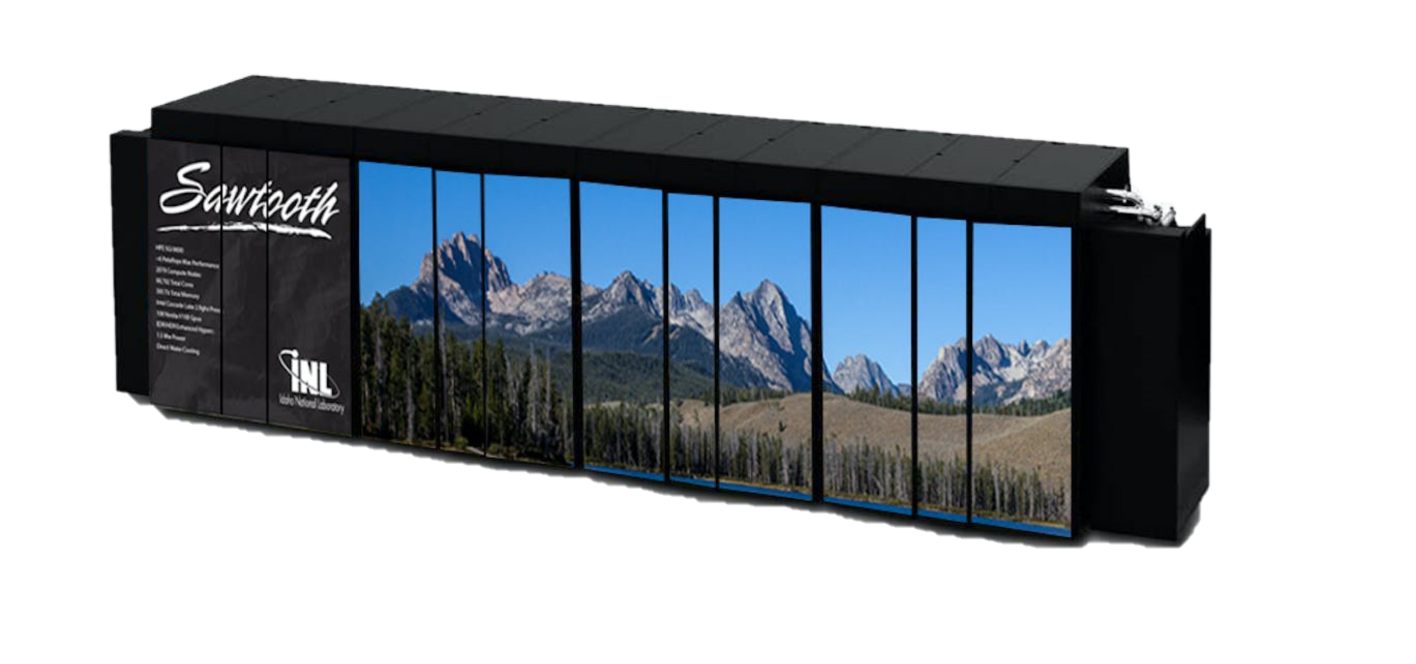
\includegraphics[height=3.5cm]{sketch/Sawtooth}};
    \node at (4.5,-3.5) {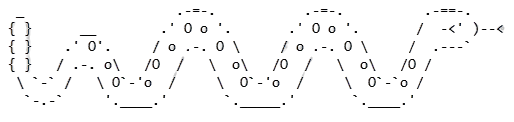
\includegraphics[height=2.5cm]{sketch/serpent}};
\end{tikzpicture}}
    \end{figure}
\end{frame}

\begin{frame}{Geometry Specification}
    \begin{columns}
    \begin{column}{0.6\textwidth}
    \begin{figure}
        \only<1>{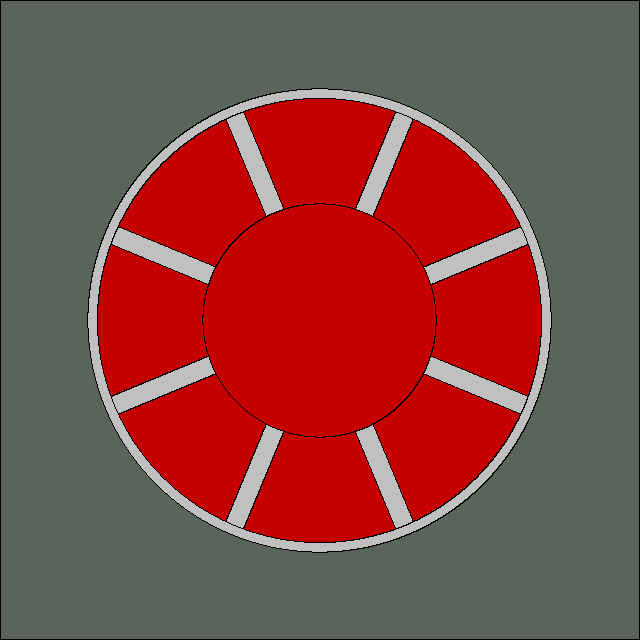
\includegraphics[width=0.95\textwidth]{Plotter/0.0/MSNB_geom2}}
        \only<2>{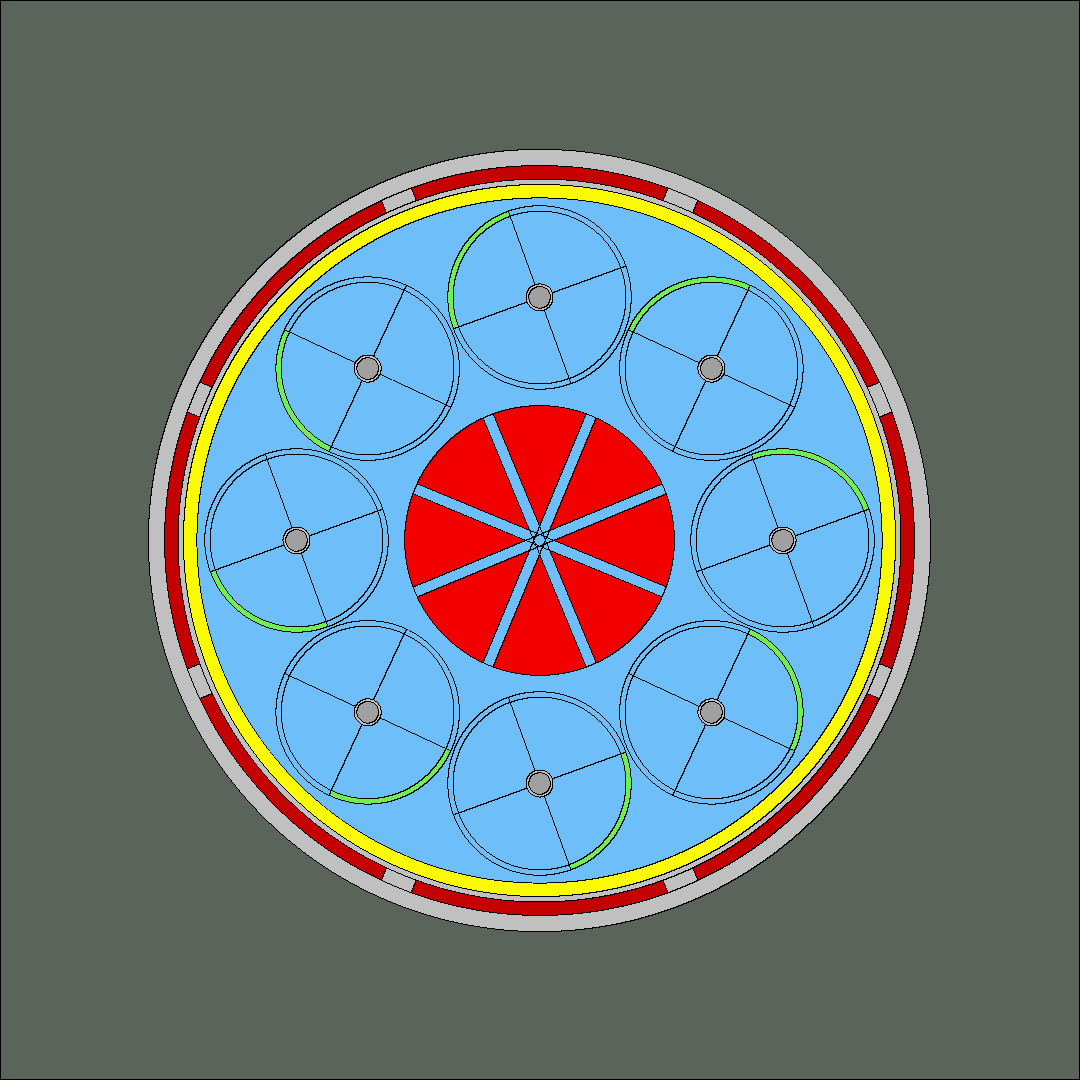
\includegraphics[width=0.95\textwidth]{Plotter/boronburn/results/10MW/MSNB_geom4}}
        \only<3>{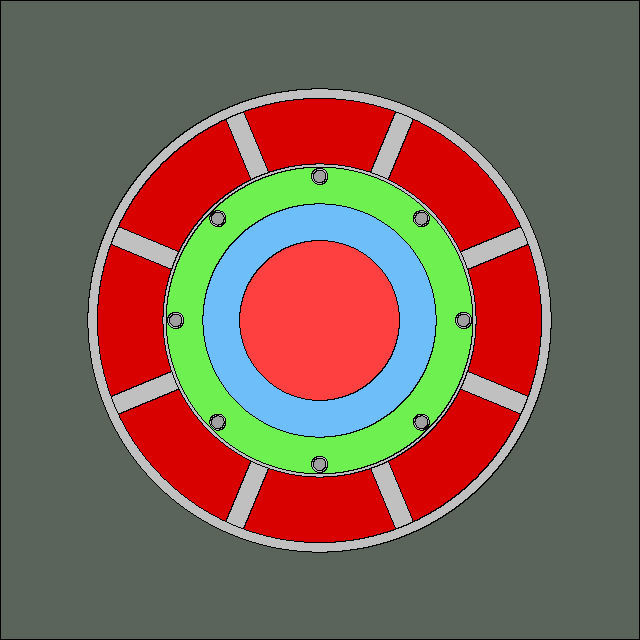
\includegraphics[width=00.95\textwidth]{Plotter/0.0/MSNB_geom6}}
        \only<4>{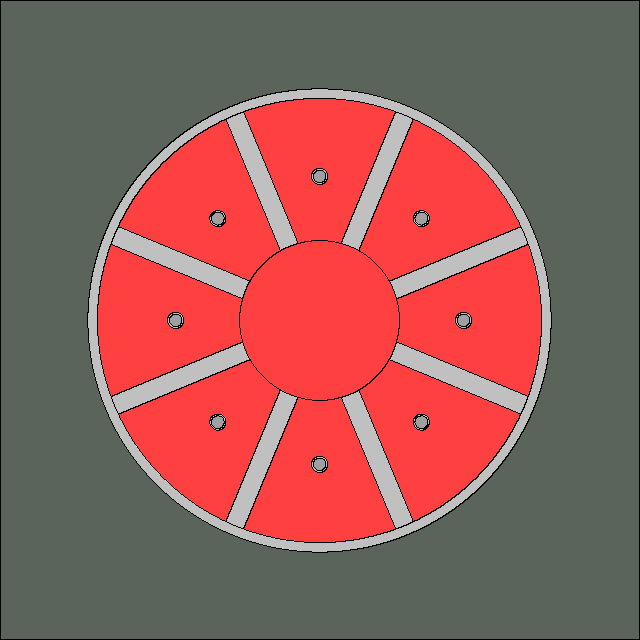
\includegraphics[width=0.95\textwidth]{Plotter/0.0/MSNB_geom8}}
        \only<5>{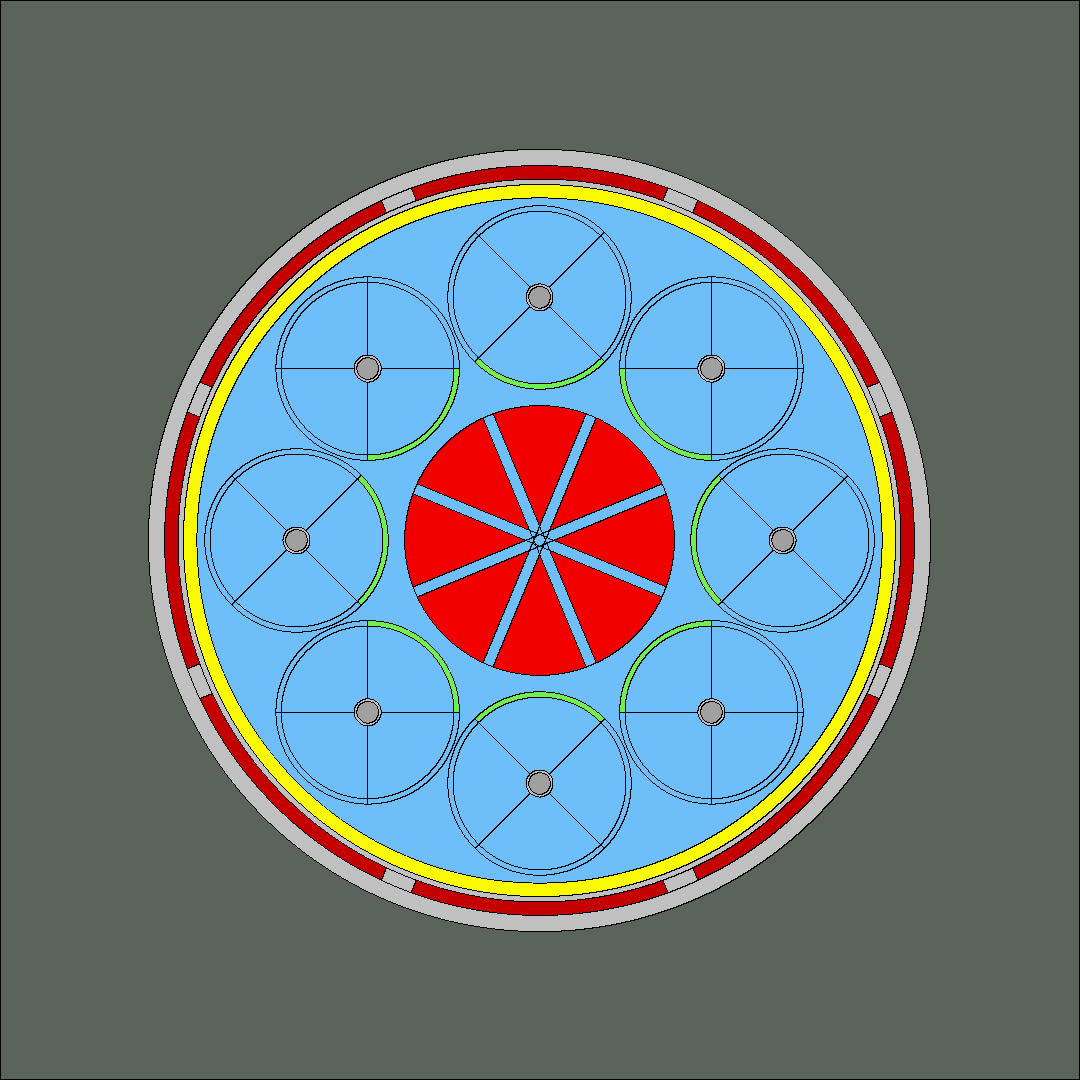
\includegraphics[width=00.95\textwidth]{Plotter/0.0/MSNB_geom4}}
        \only<6>{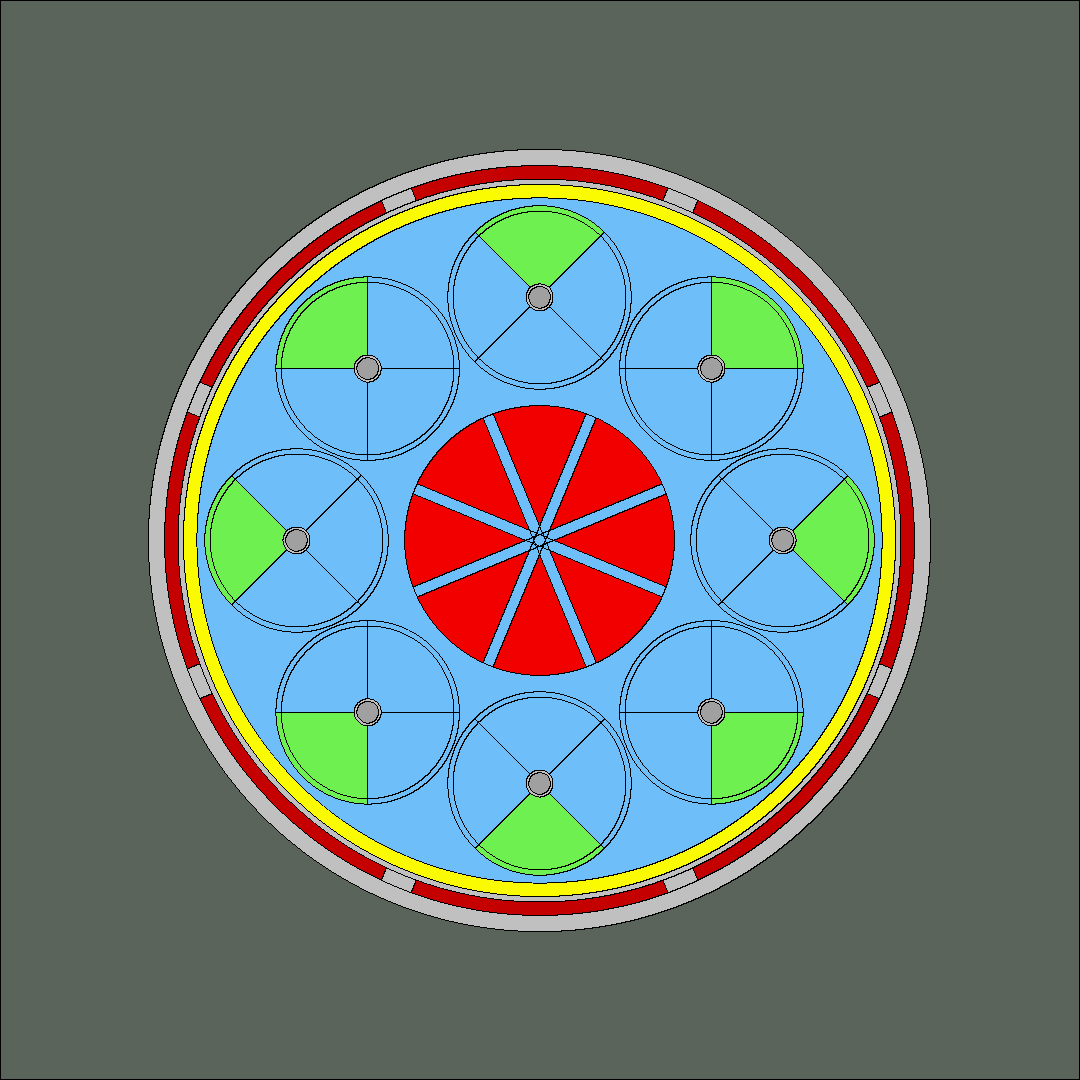
\includegraphics[width=00.95\textwidth]{Plotter/180.0/MSNB_geom4}}
        \only<7>{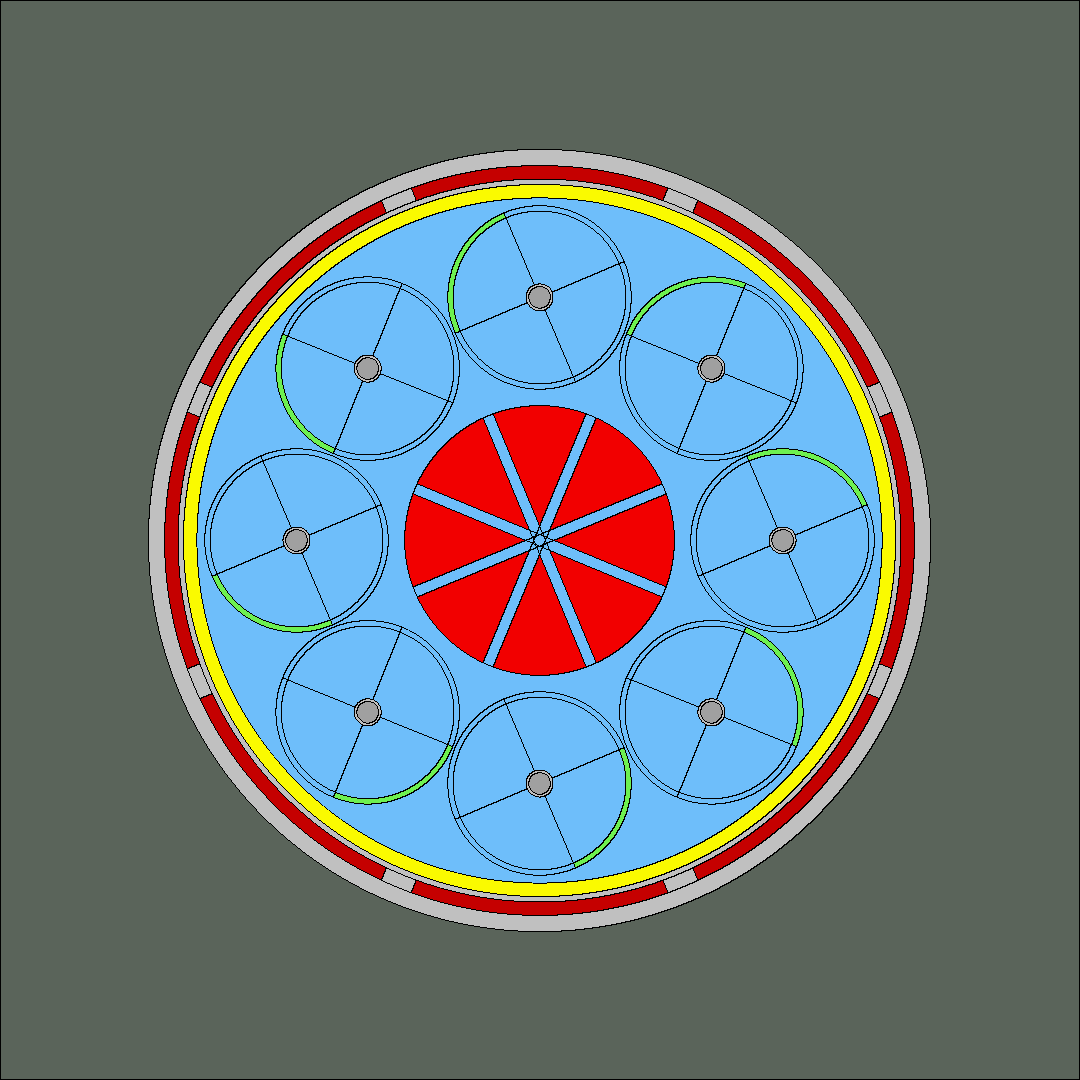
\includegraphics[width=00.95\textwidth]{Plotter/112.0/MSNB_geom4}}
    \end{figure}
    \end{column}
    \begin{column}{0.4\textwidth}
        \begin{figure}[ht!]
            \centering
            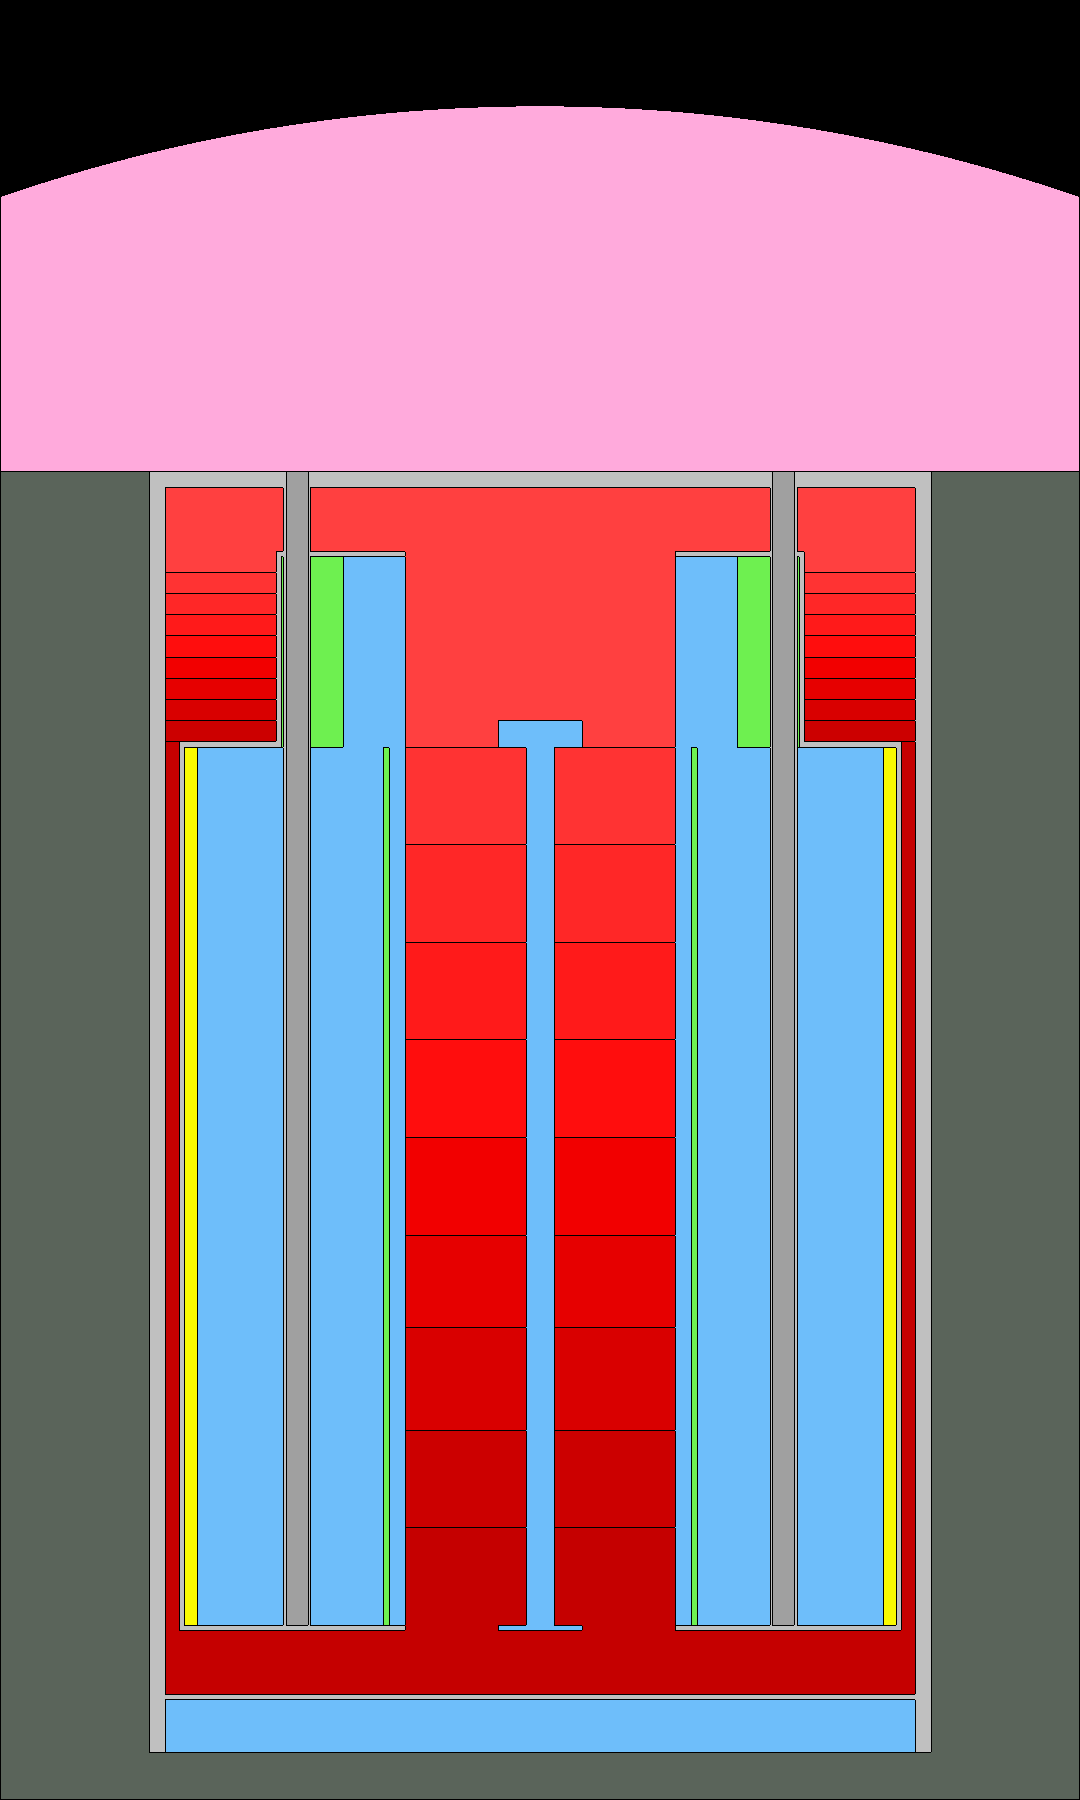
\includegraphics[height=0.95\textheight]{Plotter/0.0/MSNB_geom1.png}
        \end{figure}
    \end{column}
    \end{columns}
\end{frame}

\begin{frame}{Physics Cards}
    \begin{block}{Criticality}
        \begin{itemize}
            \item Set Pop 1,000,000 500 100 1
            \item Set Power 1e7 \%10MWth
        \end{itemize}
    \end{block}
    \begin{block}{Burn-Up}
        \begin{itemize}
            \item Set mcvol 10,000,000
            \item Set nbuf
            \item Set printm 1 1e-10
            \item Set inventory "all"
        \end{itemize}
    \end{block}
\end{frame}

\subsection{Process Simulation}
\begin{frame}{Process Simulation}
    \begin{figure}[!ht]
        \centering
        \resizebox{\textwidth}{!}{\begin{tikzpicture}
    %Pre-filter
    \draw[->] (-6,0)node[anchor=east]{$\dot{Q}_{HEX}$} -- (-4,0);
    \draw (-4,-0.5) rectangle (-3,0.5) node[pos=0.5]{$F(s)$};
    %Sum
    \draw[->] (-3,0) -- (-2,0) node[pos=0.5,anchor=south]{$\dot{Q}_{Core}^{SP}$};
    \draw (-1.75,0) circle (0.25) node{\scriptsize$-$};
    %Controller
    \draw[->] (-1.5,0) -- (-0.5,0)node[pos=0.5,anchor=south]{$e(s)$};
    \draw (-0.5,-0.5) rectangle (0.5,0.5) node[pos=0.5]{$C(s)$};
    \draw[->] (0.5,0) -- (1.5,0) node[pos=0.5,anchor=south]{$u(s)$};
    %Actuator
    \draw (1.5,-0.5) rectangle (2.5,0.5) node[pos=0.5]{$A(s)$};
    \draw[->] (2.5,0) -- (3.5,0);
    %Process
    \draw (3.5,-0.5) rectangle (4.5,0.5) node[pos=0.5]{$P(s)$};
    \draw[->] (4.5,0) -- (6.5,0) node[anchor=west]{$\dot{Q}_{Core}$};
    %Transducer
    \draw[->] (5.5,0) -- (5.5,-1.5) -- (2.5,-1.5);
    \draw (1.5,-2) rectangle (2.5,-1) node[pos=0.5]{$H(s)$} ;
    \draw[->] (1.5,-1.5) -- (-1.75,-1.5) -- (-1.75,-0.25);
    %Passive Feedback
    \draw[->] (5.5,0) -- (5.5,1.5) -- (4.5,1.5);
    \draw[->] (-5,0) -- (-5,1.5) -- (3.5,1.5);
    \draw (3.5,1) rectangle (4.5,2) node[pos=0.5]{$G(s)$};
    \draw[->] (4,1) -- (4,0.5);

    \node at (0,4) {
\includegraphics[height=2.5cm]{sketch/py}};
    \node at (5.5,4) {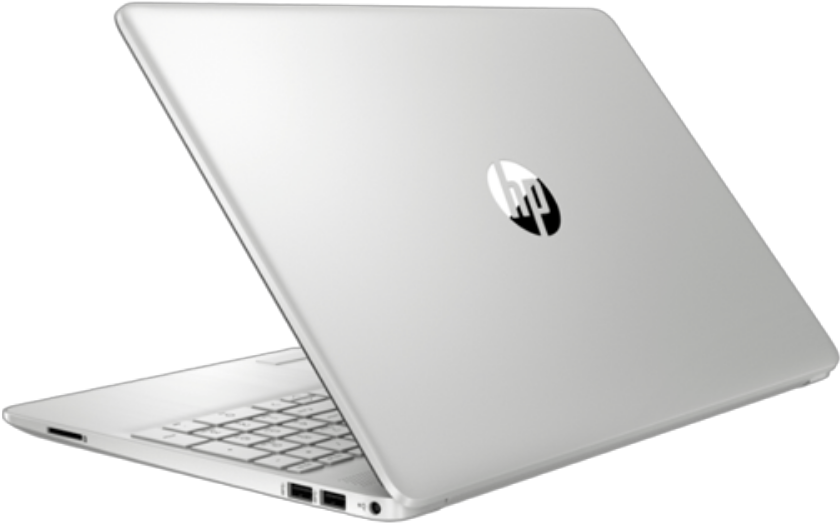
\includegraphics[height=2.5cm]{sketch/laptop}};

    \draw[red,very thick] (4,0.75) circle (1.5);
    \draw[->,red,thick] (1.4,3.5) -- (3.3,2.1);
    \draw[->,red,thick] (5.2,2.7) -- (4.7,2.1);
\end{tikzpicture}}
    \end{figure}
\end{frame}

\begin{frame}{Multi-Physics Approach}
    \begin{block}{Natural Circulation (NC)}
        \only<1>{
            Updates flow rate by equating buoyant and frictional forces
            \begin{equation*}\label{eq:saltvelo}
                v = \sqrt{\nicefrac{2gh(\varrho_{cold}-\varrho_{hot})}{\xi\varrho}}
            \end{equation*}
            }
    \end{block}
    \begin{block}{Reactor Point Kinetics (RPK)}
        \only<2>{
            Updates core power by summing passive reactivity feedback
            \begin{equation*}\label{eq:flowreac}
                \rho_f = -\frac{L}{L+H}\beta_{eff}\left(1-e^{-v\alpha_f}  \right)
            \end{equation*}
            \begin{equation*}
                \Delta\rho_T = \alpha_T\Delta T
            \end{equation*}
            \begin{equation*}
                \tau = \frac{l^{*}}{\rho}
                     +\frac{\beta_{eff}-\rho}{\lambda\rho + \dot{\rho}}
            \end{equation*}
            \begin{equation*}
                Q_{core}[t+\delta t] = Q_{core}[t] e^{\nicefrac{\delta t}{\tau}}
            \end{equation*}
        }
    \end{block}
    \begin{block}{Uniform-State Uniform-Flow (USUF)}
        \only<3>{
            Updates temperature profile based on flow rate and core/heat-exchanger powers

            \begin{equation*}
                \delta x A_x \frac{d\varrho}{dt} = v A_x(\varrho_{in}-\varrho_{out})
            \end{equation*}
            \begin{equation*}\label{eq:T2mu}
                mu_x = \varrho(T_x)\delta x A_x c_p\left(\nicefrac{T_x+T_r}{2}\right)(T_x-T_r) 
            \end{equation*}
            \begin{equation*}
                \frac{d(mu)}{dt} = mu_{enter} - mu_{exit} + Q_{c.v.}
            \end{equation*}
            \begin{equation*}
                mu[t+\delta t] = mu[t] + \delta t\frac{d(mu)}{dt}[t]
            \end{equation*}
        }
    \end{block}
\end{frame}

\begin{frame}{Logic Flow}
    \begin{figure}[!ht]
        \centering
        \resizebox{!}{\textheight}{\begin{tikzpicture}
    %blocks
    \draw (-2,-0.5) rectangle (-1,0.5) node[pos=0.5]{NC};
    \draw (1,-0.5) rectangle (2,0.5) node[pos=0.5]{RPK};
    \draw (-0.5,1.9) rectangle (0.5,2.9) node[pos=0.5]{USUF};
    
    %inner arrows
    \draw[->] (0,1.9) -- (0,0.85);
    \draw node at (0,0.7) {\tiny Temp-Profile};
    \draw[->] (-0.2,0.55) -- (-0.95,0);
    \draw[->] (0.2,0.55) -- (0.95,0);

    %outer arrows
    \draw[->] (-1.75,0.5) arc (180:112.5:2) node[midway,sloped,above]{\tiny Flow Rate};
    \draw[->] (-1.5,-0.5) arc (225:315:2) node[midway,sloped,below]{\tiny Flow Rate};
    \draw[->] (1.75,0.5) arc (0:67.5:2) node[midway,sloped,above]{\tiny Core Power};
\end{tikzpicture}}
    \end{figure}
\end{frame}

\section{Results and Analysis}
\subsection{Control-Reactivity Curve}
\begin{frame}{Control-Reactivity Curve}
    \begin{figure}[!ht]
        \centering
        \only<1>{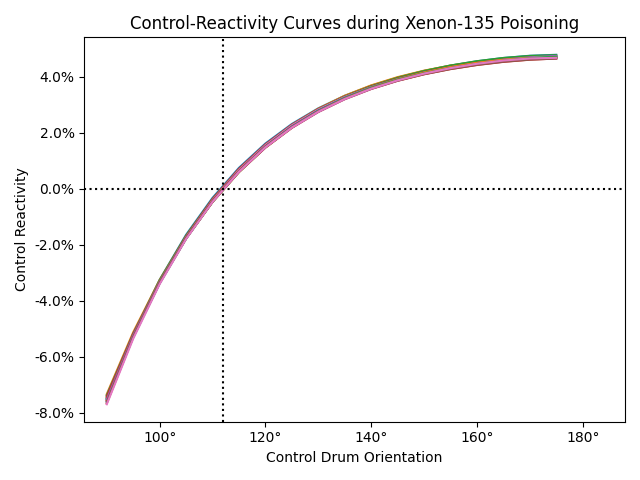
\includegraphics[height=0.9\textheight]{/CurveFits/eqXe}}
        \only<2-3>{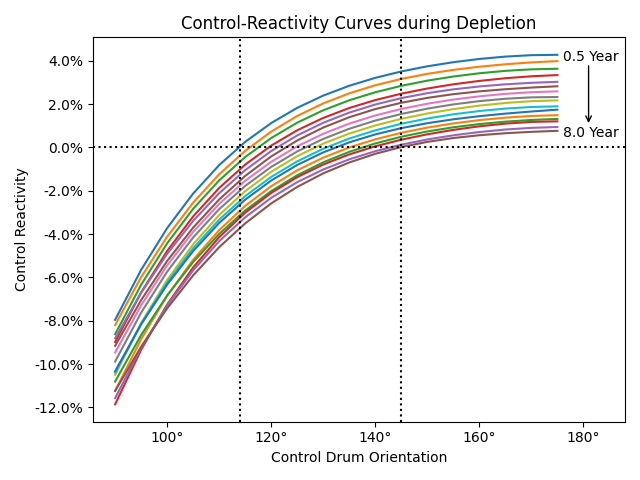
\includegraphics[height=0.9\textheight]{/CurveFits/depletion}}
    \end{figure}
    \only<3>{
        \begin{equation*}
            \rho = c_0 + c_1\theta + c_2\theta^2 + c_3\theta^3 + c_4\theta^4
        \end{equation*}
    }
\end{frame}

\begin{frame}{Curve Fits}
    \begin{table}[bh!]
        \centering\footnotesize
        \begin{tabular}{c|ccccc|cc}
        \hline
        Years & c\textsubscript{4} \sci[9] & c\textsubscript{3} \sci[6] & c\textsubscript{2} \sci[4] & c\textsubscript{1} \sci[2] & c\textsubscript{0} & root ($^o$) & slope ($pcm/^o$) \\ \hline
        0.0 & -2.797 & 1.789 & -4.361 & 4.829 & -2.009 & 111.41 & 224.24 \\
        0.5 & -2.755 & 1.755 & -4.272 & 4.732 & -1.976 & 113.69 & 203.69 \\
        1.0 & -1.838 & 1.253 & -3.253 & 3.826 & -1.682 & 115.79 & 189.71 \\
        1.5 & -2.533 & 1.632 & -3.253 & 4.507 & -1.909 & 117.38 & 175.96 \\
        2.0 & -2.418 & 1.578 & -3.930 & 4.440 & -1.895 & 119.45 & 161.06 \\\hline
        2.5 & -1.461 & 1.026 & -2.750 & 3.337 & -1.515 & 121.06 & 152.71 \\
        3.0 & -1.137 & 0.856 & -2.425 & 3.070 & -1.440 & 122.67 & 146.08 \\
        3.5 & -2.054 & 1.357 & -3.433 & 3.953 & -1.727 & 124.58 & 130.85 \\
        4.0 & -2.527 & 1.617 & -3.967 & 4.438 & -1.892 & 126.46 & 120.67 \\\hline
        4.5 & -2.869 & 1.831 & -4.460 & 4.935 & -2.081 & 128.35 & 111.30 \\
        5.0 & -2.338 & 1.520 & -3.785 & 4.291 & -1.855 & 130.55 & 102.04 \\
        5.5 & -1.471 & 1.054 & -2.852 & 3.467 & -1.585 & 132.29 & 93.34 \\
        6.0 & -2.626 & 1.702 & -4.211 & 4.729 & -2.027 & 134.96 & 83.90 \\\hline
        6.5 & -1.672 & 1.141 & -2.985 & 3.550 & -1.607 & 137.45 & 77.56 \\
        7.0 & -3.321 & 2.095 & -5.036 & 5.492 & -2.292 & 139.19 & 69.73 \\
        7.5 & -2.419 & 1.579 & -3.936 & 4.459 & -1.932 & 142.69 & 59.45 \\
        8.0 & -7.991 & 0.648 & -1.960 & 2.623 & -1.305 & 144.62 & 55.65 \\
        \end{tabular}
        \label{tab:Depletionfit}
    \end{table}
\end{frame}

\subsection{Up-Step}
\begin{frame}{Autonomous Response}
    \begin{figure}[ht!]
        \centering
        \only<1>{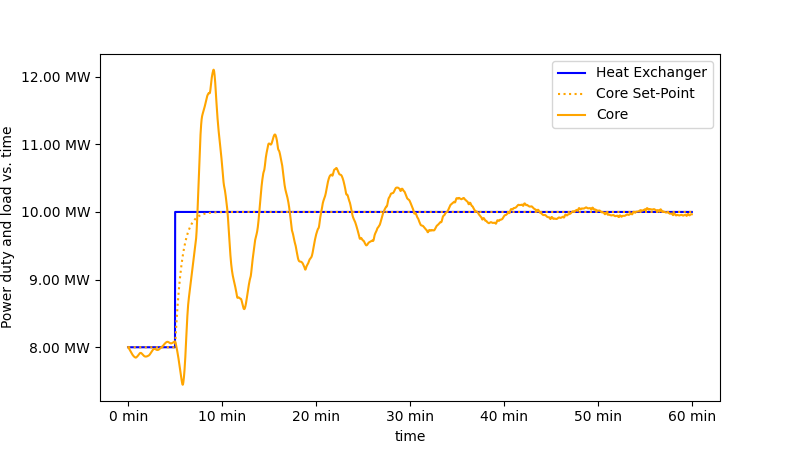
\includegraphics[width=\textwidth]{Simulator/StepUp/Auto/t_vs_Qt}}
        \only<2>{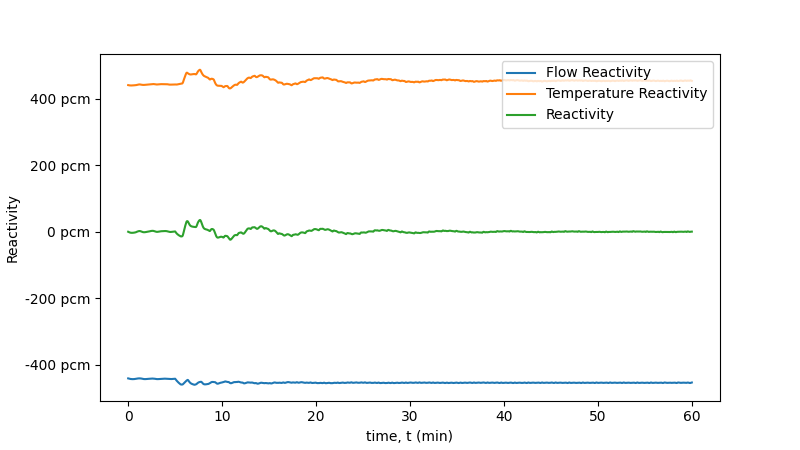
\includegraphics[width=\textwidth]{Simulator/StepUp/Auto/t_vs_reac}}
    \end{figure}
\end{frame}

\begin{frame}{Controller Tuning}
    \begin{block}{Ziegler Nichols Tuning Methodology}
        \only<1-2>{
            \begin{itemize}
                \item P-Only Control
                \item Increase gain until sustained oscillations
                \item<2> Ultimate gain - 3 $\times$ 10\textsuperscript{-4} degree/kW
                \item<2> Ultimate period - 45 seconds
            \end{itemize}
        }
    \end{block}
    \begin{block}{Controller Parameters}
        \only<3->{
            \begin{itemize}
                \item Controller gain - 1.35 $\times$ 10\textsuperscript{-4} degree/kW at 0 years 
                \item Controller-Actuator gain - 30.3 pcm/MW
                \item Integral time-constant - 37.5 seconds
                \item Derivative time-constant - 0 sec
                \item Controller bias - 111.41$^o$ at zero years, 144.62$^o$ at eight years
            \end{itemize}
        }
        
    \end{block}
\end{frame}

\begin{frame}{Controlled Response}
    \begin{figure}[ht!]
        \centering
        \only<1>{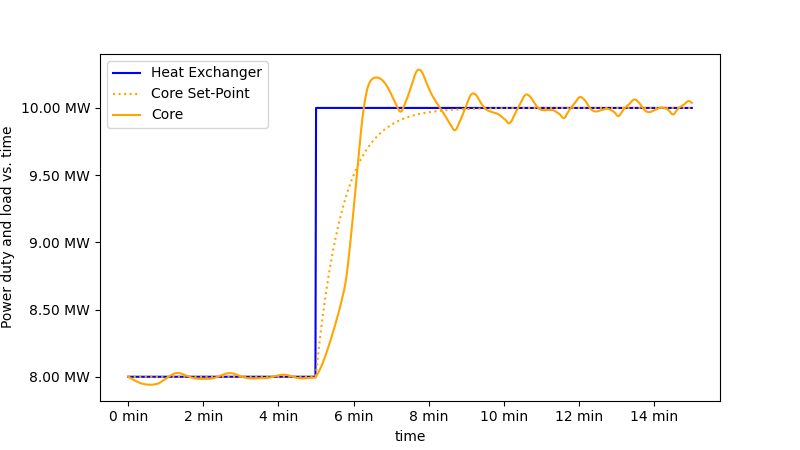
\includegraphics[width=\textwidth]{Simulator/StepUp/Control/t_vs_Qt}}
        \only<2>{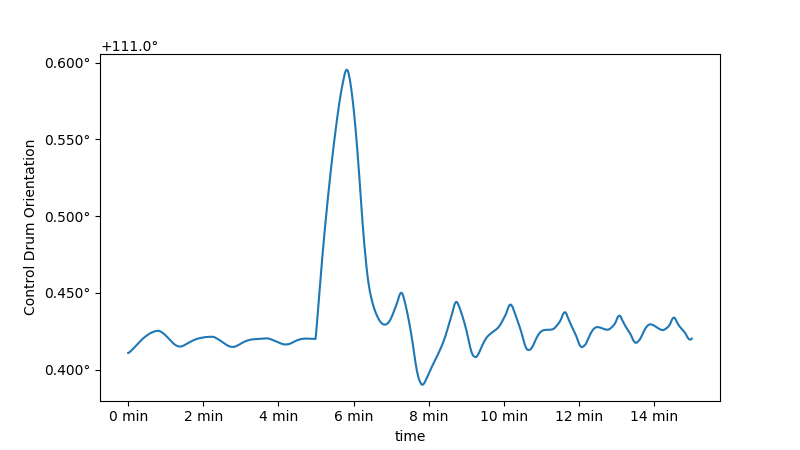
\includegraphics[width=\textwidth]{Simulator/StepUp/Control/t_vs_angle}}
    \end{figure}
\end{frame}

\subsection{Down-Step}
\begin{frame}{Autonomous Response}
    \begin{figure}[ht!]
        \centering
        \only<1>{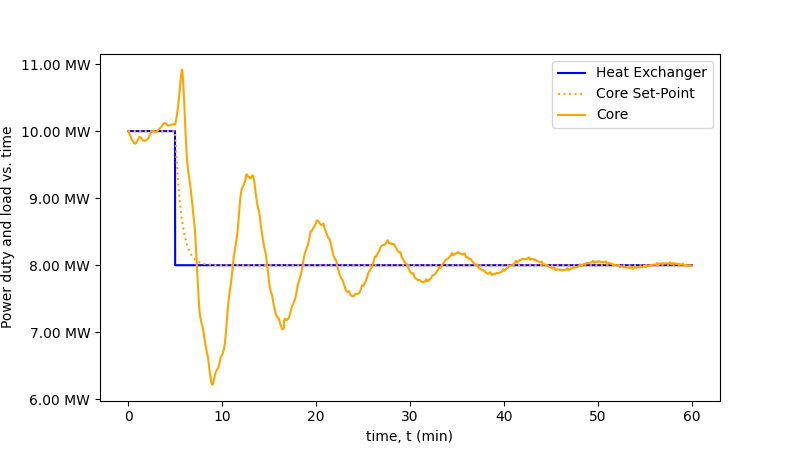
\includegraphics[width=\textwidth]{Simulator/StepDown/Auto/t_vs_Qt}}
        \only<2>{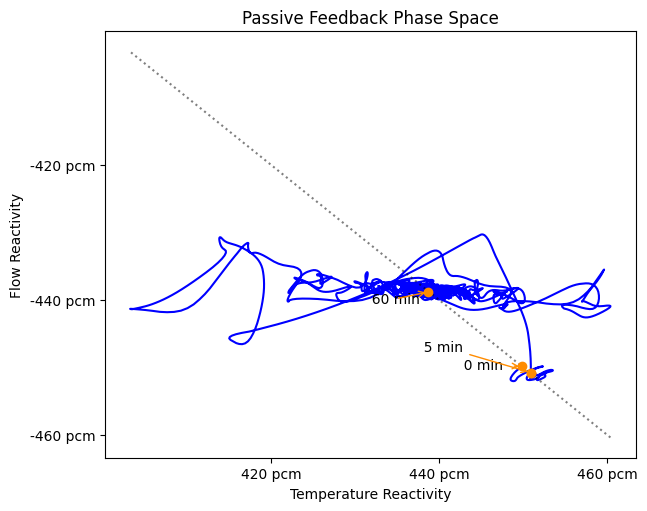
\includegraphics[width=\textwidth]{Simulator/StepDown/Auto/auto_reac_phase}}
    \end{figure}
\end{frame}

\begin{frame}{Controlled Response}
    \begin{figure}[ht!]
        \centering
        \only<1>{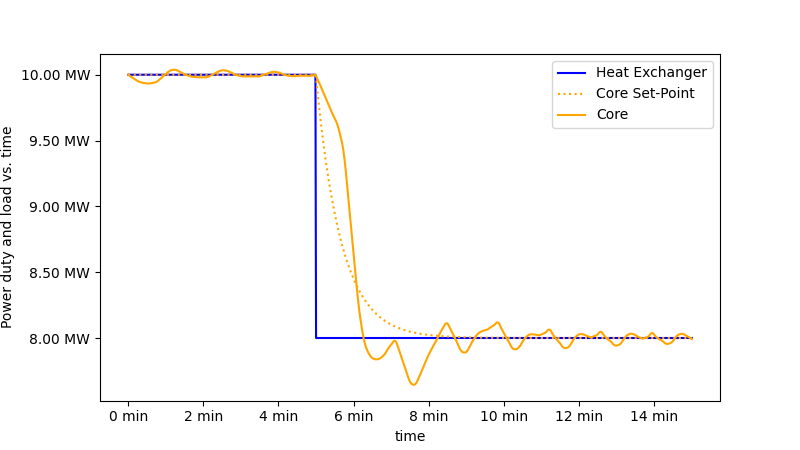
\includegraphics[width=\textwidth]{Simulator/StepDown/Control/t_vs_Qt}}
        \only<2>{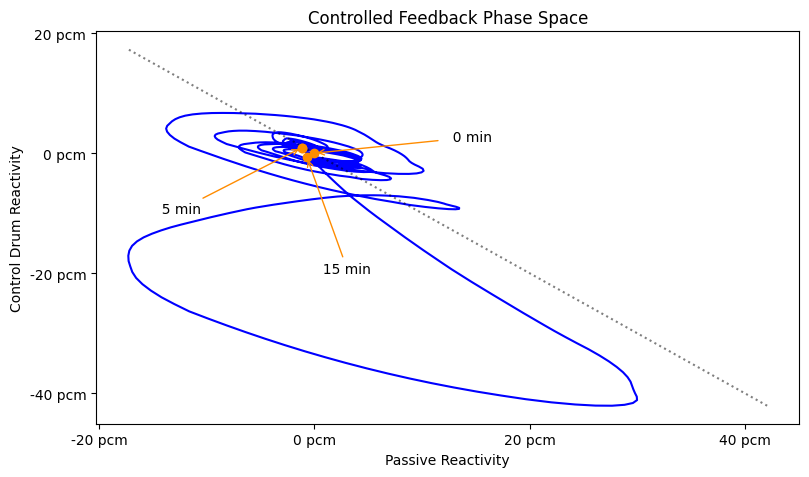
\includegraphics[width=\textwidth]{Simulator/StepDown/Control/contr_reac_phase}}
    \end{figure}
\end{frame}

\subsection{Start-Up}
\begin{frame}{Autonomous Response}
    \begin{figure}[ht!]
        \centering
        \only<1>{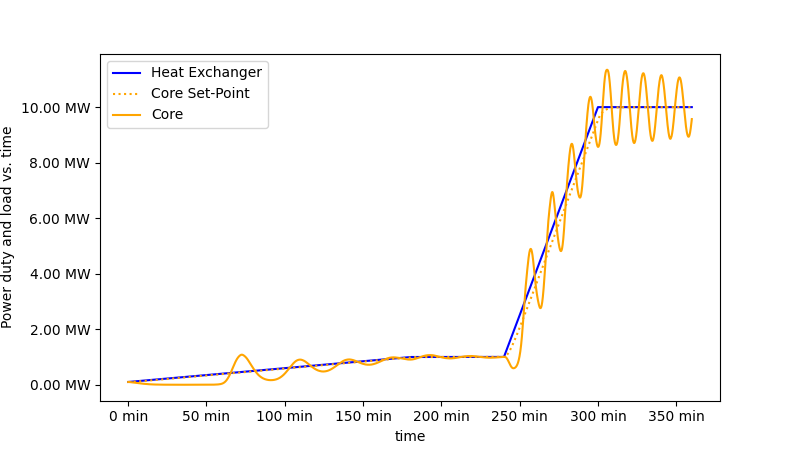
\includegraphics[width=\textwidth]{Simulator/StartUp/Auto/t_vs_Qt}}
        \only<2>{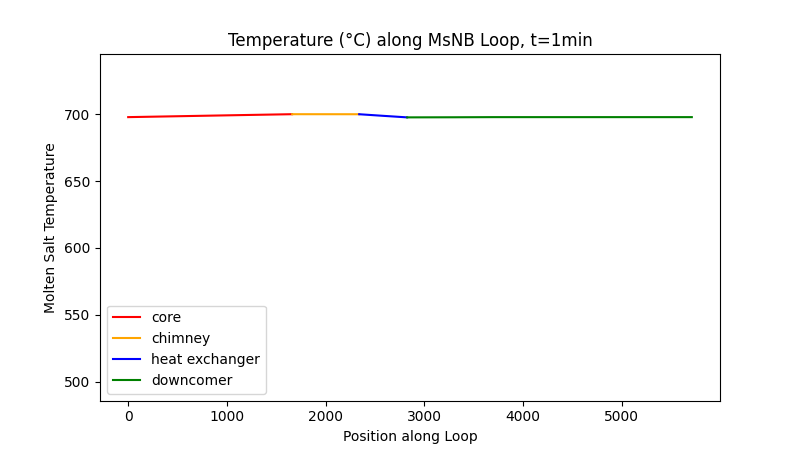
\includegraphics[width=\textwidth]{Simulator/StartUp/Auto/animateTx_t/t-1}}
        \only<3>{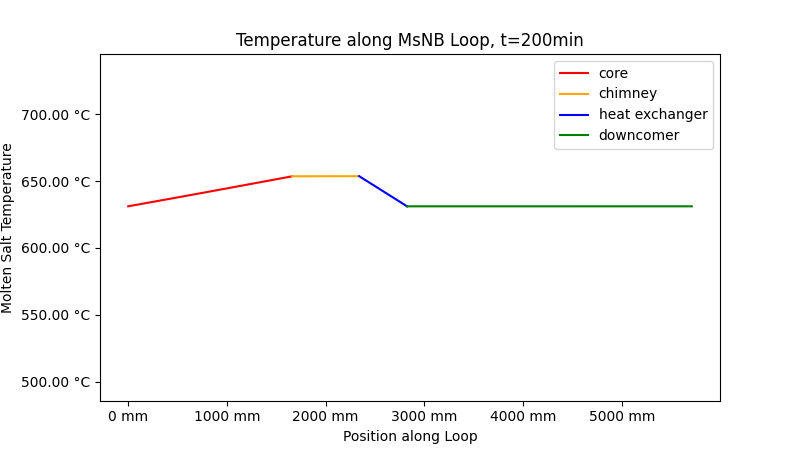
\includegraphics[width=\textwidth]{Simulator/StartUp/Auto/animateTx_t/t-200}}
        \only<4>{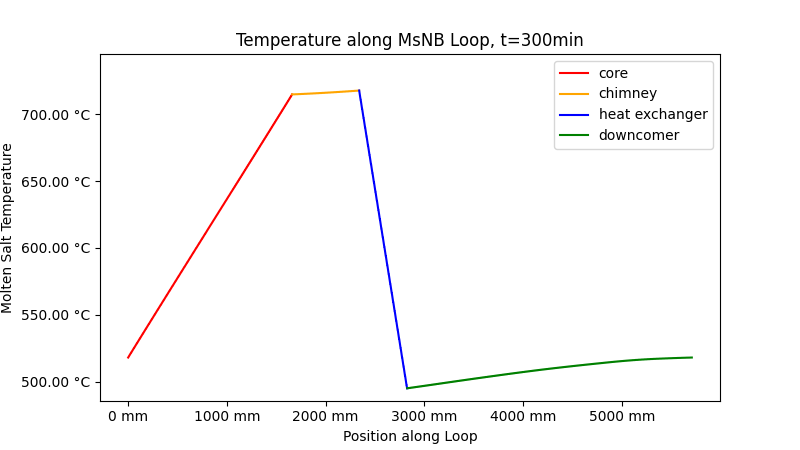
\includegraphics[width=\textwidth]{Simulator/StartUp/Auto/animateTx_t/t-300}}
        \only<5>{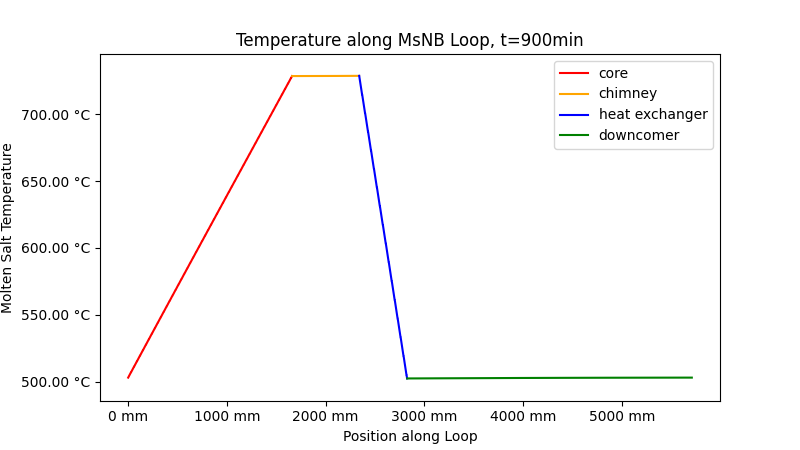
\includegraphics[width=\textwidth]{Simulator/StartUp/Auto/animateTx_t/t-900}}
    \end{figure}
\end{frame}

\begin{frame}{Controlled Response}
    \begin{figure}[ht!]
        \centering
        \only<1>{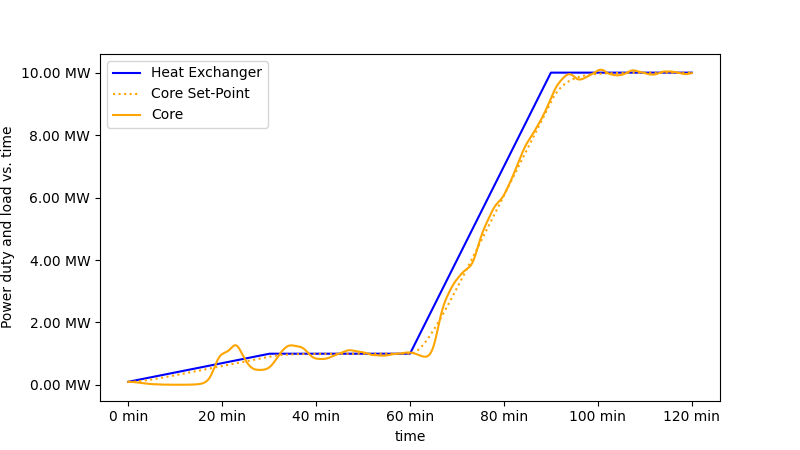
\includegraphics[width=\textwidth]{Simulator/StartUp/Control/t_vs_Qt}}
        \only<2>{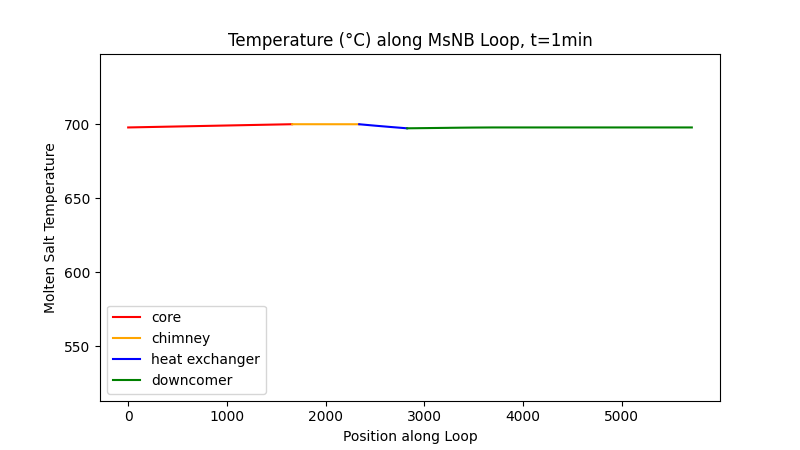
\includegraphics[width=\textwidth]{Simulator/StartUp/Control/animateTx_t/t-1}}
        \only<3>{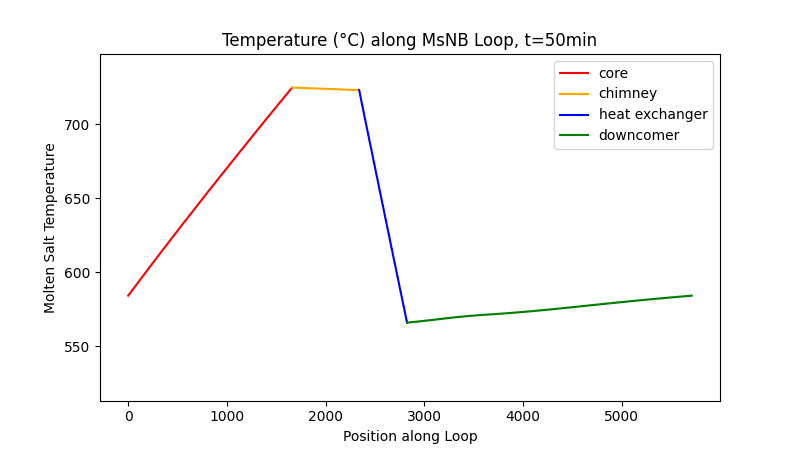
\includegraphics[width=\textwidth]{Simulator/StartUp/Control/animateTx_t/t-50}}
        \only<4>{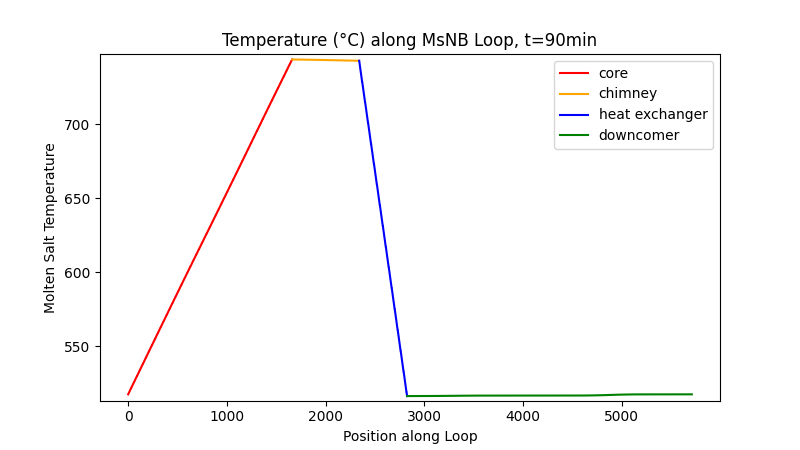
\includegraphics[width=\textwidth]{Simulator/StartUp/Control/animateTx_t/t-90}}
        \only<5>{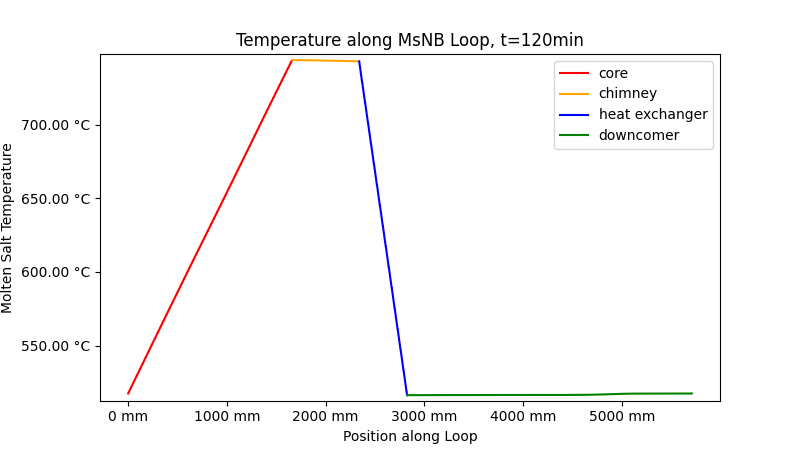
\includegraphics[width=\textwidth]{Simulator/StartUp/Control/animateTx_t/t-120}}
    \end{figure}
\end{frame}


\subsection{Shut-Down}
\begin{frame}{Autonomous Response}
    \begin{figure}[ht!]
        \centering
        \only<1>{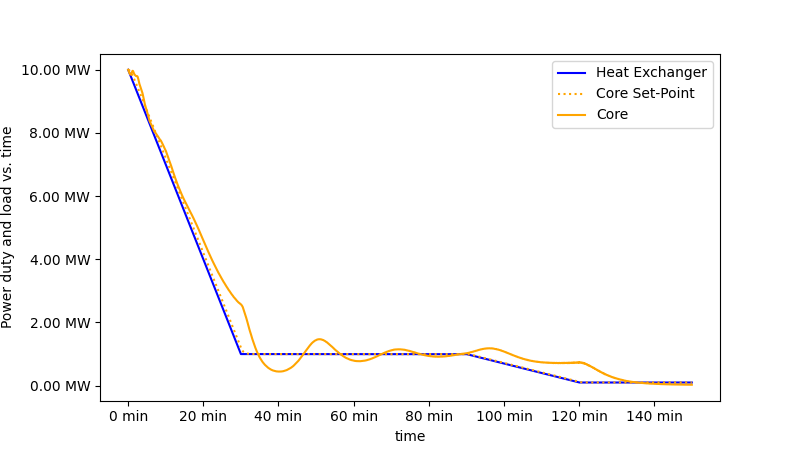
\includegraphics[width=\textwidth]{Simulator/ShutDown/Auto/t_vs_Qt}}
        \only<2>{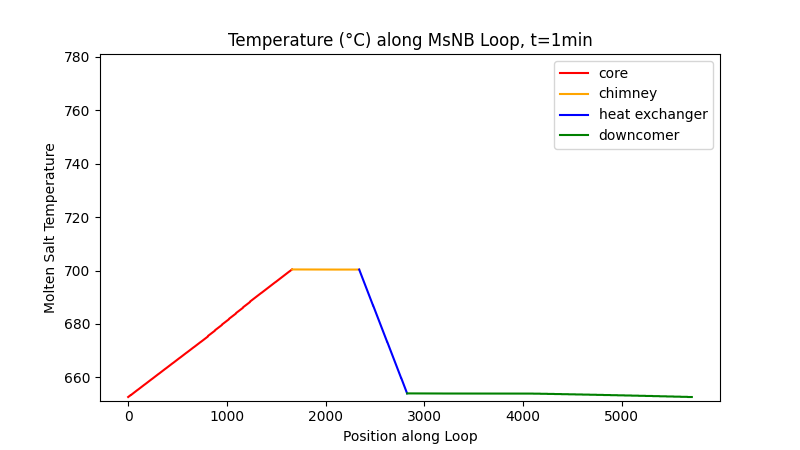
\includegraphics[width=\textwidth]{Simulator/ShutDown/Auto/animateTx_t/t-1}}
        \only<3>{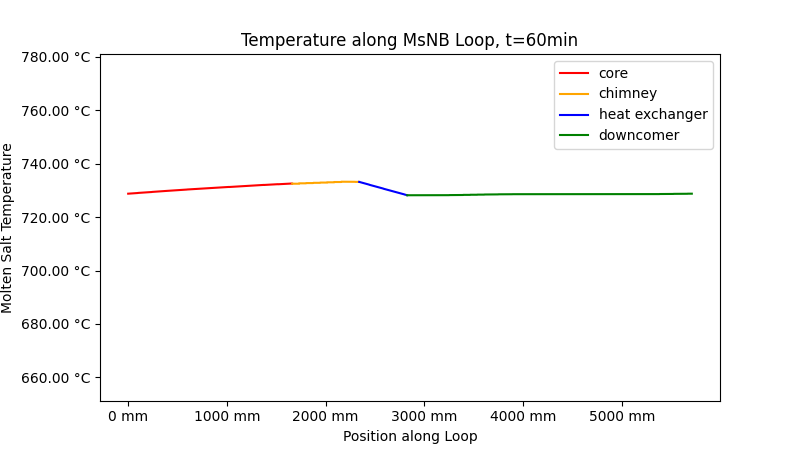
\includegraphics[width=\textwidth]{Simulator/ShutDown/Auto/animateTx_t/t-60}}
        \only<4>{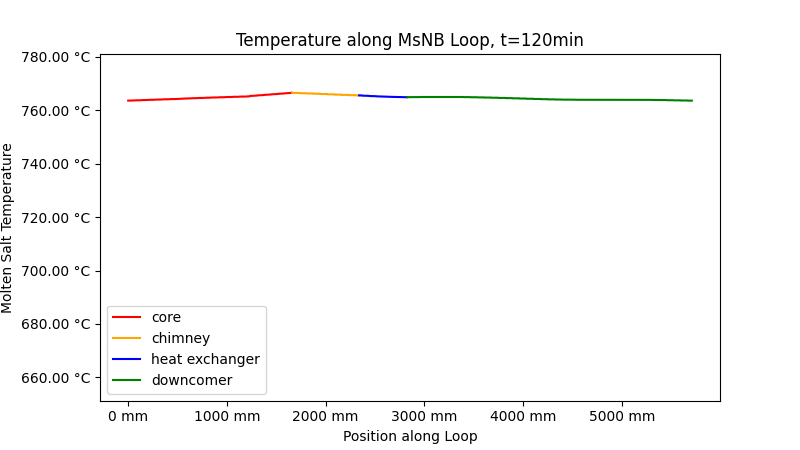
\includegraphics[width=\textwidth]{Simulator/ShutDown/Auto/animateTx_t/t-120}}
        \only<5>{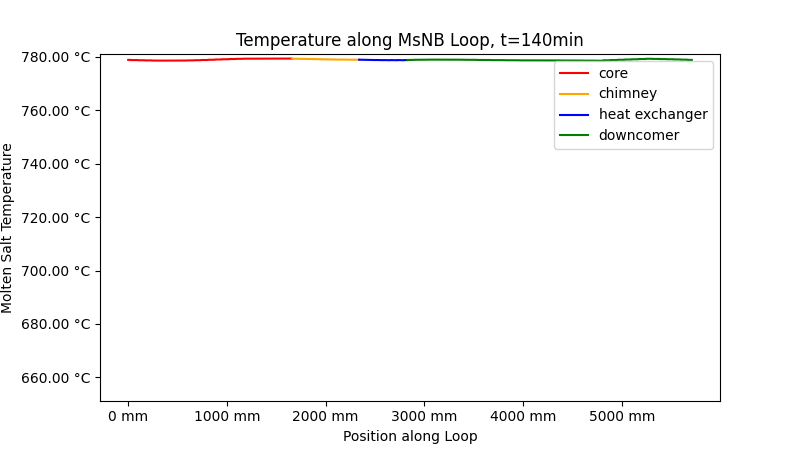
\includegraphics[width=\textwidth]{Simulator/ShutDown/Auto/animateTx_t/t-140}}
    \end{figure}
\end{frame}

\begin{frame}{Controlled Response}
    \begin{figure}[ht!]
        \centering
        \only<1>{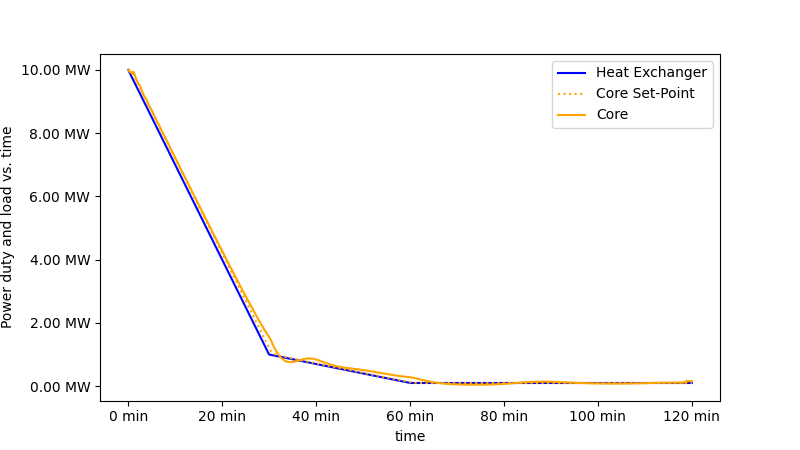
\includegraphics[width=\textwidth]{Simulator/ShutDown/Control/t_vs_Qt}}
        \only<2>{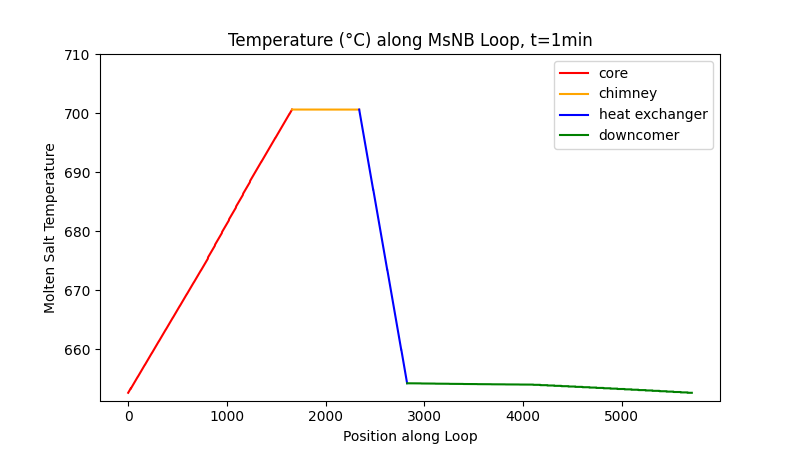
\includegraphics[width=\textwidth]{Simulator/ShutDown/Control/animateTx_t/t-1}}
        \only<3>{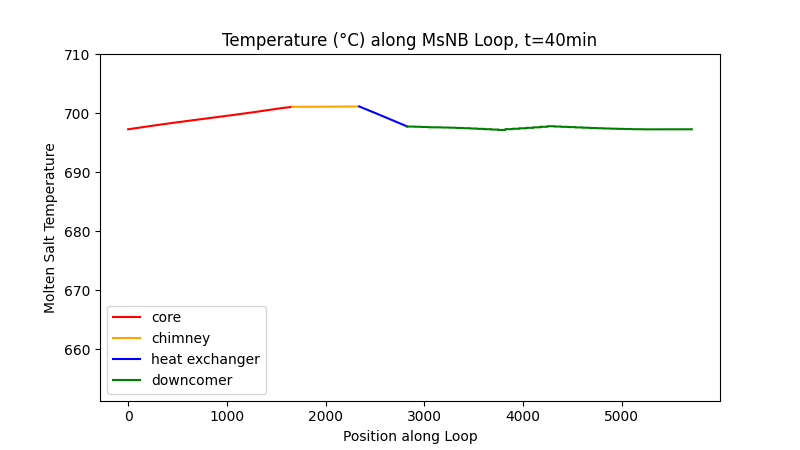
\includegraphics[width=\textwidth]{Simulator/ShutDown/Control/animateTx_t/t-40}}
        \only<4>{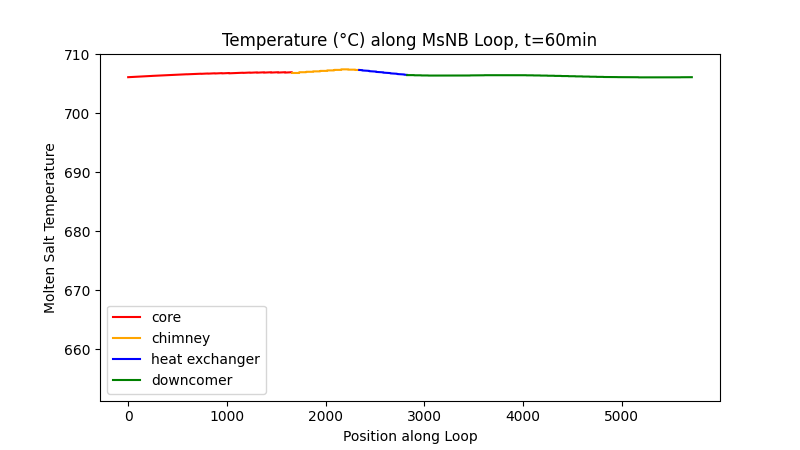
\includegraphics[width=\textwidth]{Simulator/ShutDown/Control/animateTx_t/t-60}}
        \only<5>{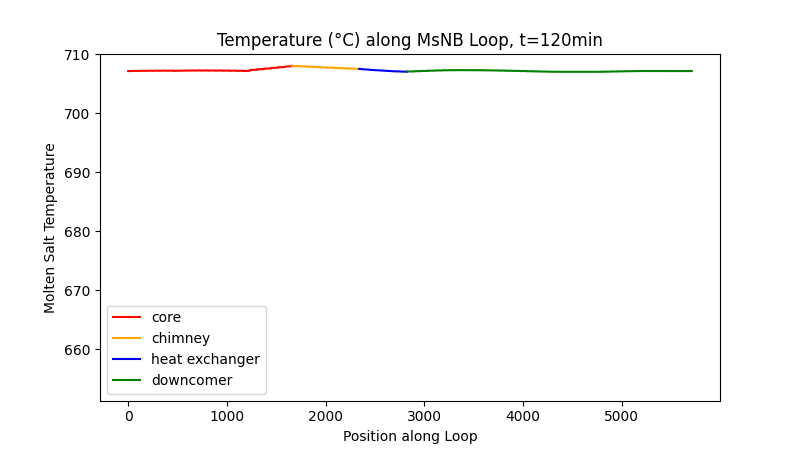
\includegraphics[width=\textwidth]{Simulator/ShutDown/Control/animateTx_t/t-120}}
    \end{figure}
\end{frame}

\subsection{Demand-Response}
\begin{frame}{Autonomous Response}
    \begin{figure}[ht!]
        \centering
        \only<1>{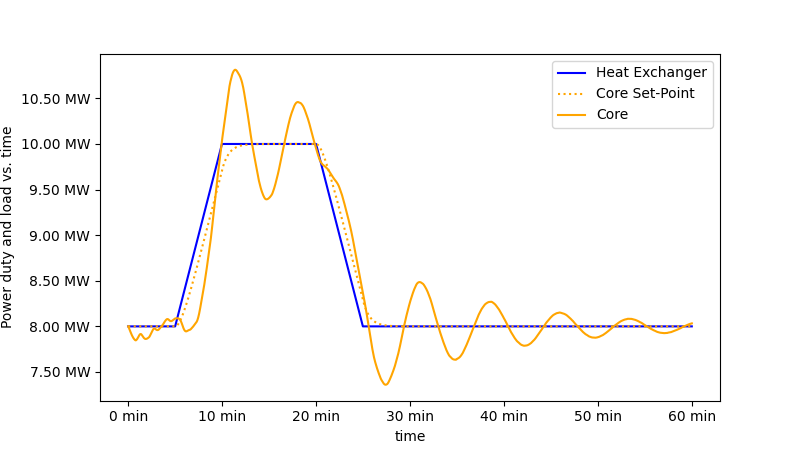
\includegraphics[width=\textwidth]{Simulator/DemandResponse/Auto/t_vs_Qt}}
        \only<2>{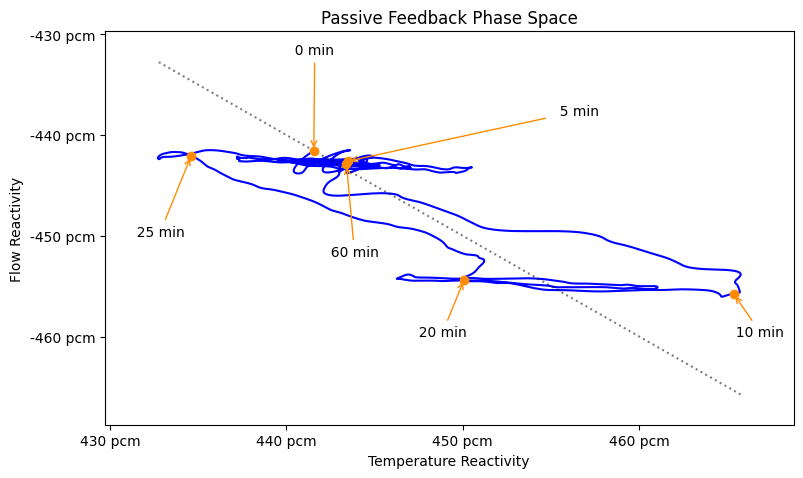
\includegraphics[width=\textwidth]{Simulator/DemandResponse/Auto/auto_reac_phase}}
    \end{figure}
\end{frame}

\begin{frame}{Controlled Response}
    \begin{figure}[ht!]
        \centering
        \only<1>{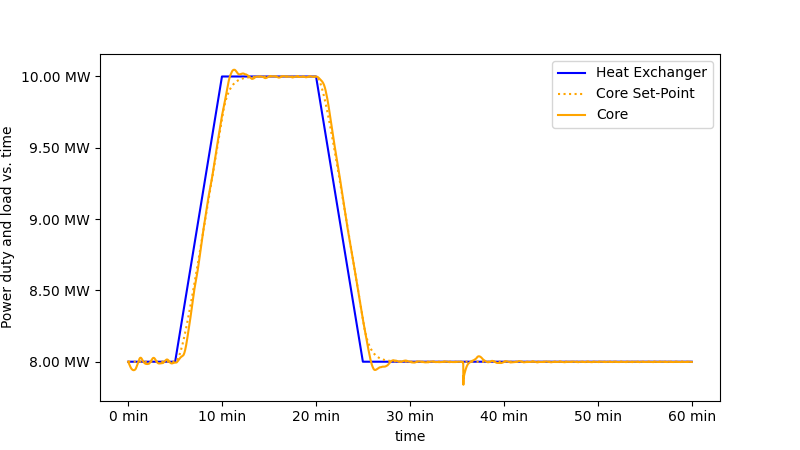
\includegraphics[width=\textwidth]{Simulator/DemandResponse/Control/t_vs_Qt}}
        \only<2>{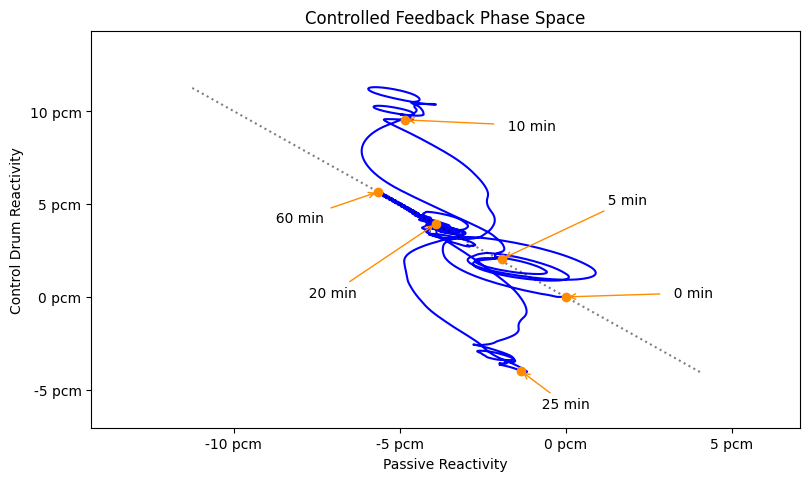
\includegraphics[width=\textwidth]{Simulator/DemandResponse/Control/contr_reac_phase}}
    \end{figure}
\end{frame}


\section{Conclusions}
\begin{frame}{Conclusions}
    \begin{block}{Summary of Models Completed}
        \only<1>{
            \begin{itemize}
                \item Alternating criticality and burn-up models were developed in Serpent 2 to study the evolution of the control-reactivity curve over the life of the MSNB
        \item Mass and energy conservation were coupled to reactor point kinetics in a Python 3.10 code to predict the flow rate and power of the \acs{msnb}
        \item Time and spatial advancement routine simulates heat and mass advection according to uniform-state uniform-flow
        \item A pre-filter reshapes the heat exchanger demand
        \item A PI controller compliments the passive feedback mechanisms inherent to the \acs{msnb}
            \end{itemize}
        }
        \begin{block}{Results In-Brief}
            \only<2>{
                \begin{itemize}
                    \item The \acs{msnb} design studied in this work has an excess reactivity of 4.834\% at hot-standby
                    \item After 8 full-power years, the \acs{msnb} fuel is depleted enough to no longer provide enough excess reactivity for effective operation
                    \item The autonomous response is stable, but significantly under-damped for 20\% step functions and ramp functions of up to 400 kW/min
                    \item The PI controller with improves the settling time by an order of magnitude for step functions, and essentially eliminates overshoot for ramp functions
                    \item With a robust controller, the MSNB is suitable for load-following
                \end{itemize}
            }
            
        \end{block}
    \end{block}
\end{frame}

\begin{frame}{Acknowledgements}
    \centering
    This work and my coursework is being completed under a Graduate Fellowship funded by \acf{nrc}.

    This research made use of the resources of the High Performance Computing Center at Idaho National Laboratory, which is supported by the Office of Nuclear Energy of the U.S. Department of Energy and the Nuclear Science User Facilities under Contract No. DE-AC07-05ID14517.
\end{frame}

\begin{frame}[plain]{}
    \noside
    
\includegraphics[height=0.9\textheight]{logo}
    \vfill
\end{frame}

\begin{frame}[allowframebreaks]{References}
    \bibliographystyle{./rcs/neup}
    \footnotesize
    \bibliography{./rcs/References}
\end{frame}

%%%%%%%%%%%%%%%%%%%%%%%%%%%%%%%%%%%%%%%%%%%%%%%%%%%%%%%%%%%%%%%%%%%%%%%%%%%%%%%%%%%%%%%%%%%%%%%%%%%%%%%%%%%%%%%%%%%%%%%%%%%%%%%%%%%%%%%%%%%%%%%%%%%%%%%%%%%%%%%%%%%%%%%%%%%%%%%%%%%%%%%%%%%%%

\begin{comment}
    \begin{frame}{Fission Product Poisoning}
    \only<1>{\begin{figure}[h]\centering
        \resizebox{0.9\textwidth}{!}{\begin{tikzpicture}
    %Xenon
    \filldraw[green] circle (16cm);
    \draw node[scale=4] at (0,14) {$\sigma_a^{^{135}Xe} = 430 kb$};
    %Iodine
    \filldraw[blue] (-9,9) circle (0.1cm);
    \draw node[scale=4] at (-9,7) {$\sigma_a^{^{135}I} = 260 mb$};
    %Uranium
    \filldraw[red] (7,7) circle (0.33cm);
    \draw node[scale=4] at (7,5.5) {$\sigma_f^{^{235}U} = 180 b$};
    %Arrows 
    % \draw[->,line width=1mm] (6.5,7) -- (-8.5,9) node[scale=2,midway,above,sloped] {$\gamma_{I} = 6.39\%$};
    % \draw[->,line width=1mm] (6.5,7.5) -- (-4,12.5) node[scale=2,midway,above,sloped] {$\gamma_{Xe} = 0.24\%$};
    % \draw[->,line width=1mm] (-8.5,9.5) -- (-4.5,12.5) node[scale=2,midway,above,sloped] {$t_{\nicefrac{1}{2}} = 6.7 hr$};
    % %Equations
    % \draw node[scale=2.5] at (0,2) {$\frac{dI}{dt} =
    % \underbrace{\gamma_{I}\Sigma_{f}^{F}{\phi}(t)}_{\text{Fission Yield}}-\underbrace{\lambda_{I}I(t)}_{\text{Beta Decay}}$};
    % \draw node[scale=2.5] at (0,-1) {$\frac{dXe}{dt} =
    %     \underbrace{\gamma_{Xe}\Sigma_{f}^{F}{\phi}(t)}_{\text{Fission Yield}}+\underbrace{\lambda_{I}I(t)}_{\text{Precursor Decay}}-\underbrace{\lambda_{Xe}Xe(t)}_{\text{Beta Decay}}-\underbrace{Xe(t)\sigma_{a}^{Xe}{\phi}(t)}_{\text{Radiative Capture}}$};
\end{tikzpicture}

}
        \end{figure}}
    \only<2>{\begin{figure}[h]\centering
        \resizebox{0.9\textwidth}{!}{\begin{tikzpicture}
    %Xenon
    \filldraw[green] circle (16cm);
    \draw node[scale=4] at (0,14) {$\sigma_a^{^{135}Xe} = 430 kb$};
    %Iodine
    \filldraw[blue] (-9,9) circle (0.1cm);
    \draw node[scale=4] at (-9,7) {$\sigma_a^{^{135}I} = 260 mb$};
    %Uranium
    \filldraw[red] (7,7) circle (0.33cm);
    \draw node[scale=4] at (7,5.5) {$\sigma_f^{^{235}U} = 180 b$};
    %Arrows 
    \draw[->,line width=1mm] (6.5,7) -- (-8.5,9) node[scale=2,midway,above,sloped] {$\gamma_{I} = 6.39\%$};
    \draw[->,line width=1mm] (6.5,7.5) -- (-4,12.5) node[scale=2,midway,above,sloped] {$\gamma_{Xe} = 0.24\%$};
    \draw[->,line width=1mm] (-8.5,9.5) -- (-4.5,12.5) node[scale=2,midway,above,sloped] {$t_{\nicefrac{1}{2}} = 6.7 hr$};
    % %Equations
    % \draw node[scale=2.5] at (0,2) {$\frac{dI}{dt} =
    % \underbrace{\gamma_{I}\Sigma_{f}^{F}{\phi}(t)}_{\text{Fission Yield}}-\underbrace{\lambda_{I}I(t)}_{\text{Beta Decay}}$};
    % \draw node[scale=2.5] at (0,-1) {$\frac{dXe}{dt} =
    %     \underbrace{\gamma_{Xe}\Sigma_{f}^{F}{\phi}(t)}_{\text{Fission Yield}}+\underbrace{\lambda_{I}I(t)}_{\text{Precursor Decay}}-\underbrace{\lambda_{Xe}Xe(t)}_{\text{Beta Decay}}-\underbrace{Xe(t)\sigma_{a}^{Xe}{\phi}(t)}_{\text{Radiative Capture}}$};
\end{tikzpicture}

}
        \end{figure}}
    \only<3>{\begin{figure}[h]\centering
        \resizebox{0.9\textwidth}{!}{\begin{tikzpicture}[draw=gray,color=gray]
    \clip (-17,17) rectangle (17,-3);
    %Xenon
    \filldraw[green] circle (16cm);
    \draw node[scale=4] at (0,14) {$\sigma_a^{^{135}Xe} = 430 kb$};
    %Iodine
    \filldraw[blue!50!] (-9,9) circle (0.1cm);
    \draw node[scale=4] at (-9,7) {$\sigma_a^{^{135}I} = 260 mb$};
    %Uranium
    \filldraw[red!50!] (7,7) circle (0.33cm);
    \draw node[scale=4] at (7,5.5) {$\sigma_f^{^{235}U} = 180 b$};
    %Arrows 
    \draw[->,line width=1mm] (6.5,7) -- (-8.5,9) node[scale=2,midway,above,sloped] {$\gamma_{I} = 6.39\%$};
    \draw[->,line width=1mm] (6.5,7.5) -- (-4,12.5) node[scale=2,midway,above,sloped] {$\gamma_{Xe} = 0.24\%$};
    \draw[->,line width=1mm] (-8.5,9.5) -- (-4.5,12.5) node[scale=2,midway,above,sloped] {$t_{\nicefrac{1}{2}} = 6.7 hr$};
    %Equations
    \draw node[scale=2.5,color=black] at (0,2) {$\frac{dI}{dt} =
    \underbrace{\gamma_{I}\Sigma_{f}^{F}{\phi}(t)}_{\text{Fission Yield}}-\underbrace{\lambda_{I}I(t)}_{\text{Beta Decay}}$};
    \draw node[scale=2.5,color=black] at (0,-1) {$\frac{dXe}{dt} = \underbrace{\lambda_{I}I(t)}_{\text{Precursor Decay}}+\underbrace{\gamma_{Xe}\Sigma_{f}^{F}{\phi}(t)}_{\text{Fission Yield}}-\underbrace{\lambda_{Xe}Xe(t)}_{\text{Beta Decay}}-\underbrace{Xe(t)\sigma_{a}^{Xe}{\phi}(t)}_{\text{Radiative Capture}}$};
\end{tikzpicture}

}
        \end{figure}}
\end{frame}

\setbeamercolor{background canvas}{bg=White}
\begin{frame}{Xenon Dynamics}
    \begin{columns}
        \begin{column}{0.5\textwidth}
            \begin{figure}[ht!]
                \centering
                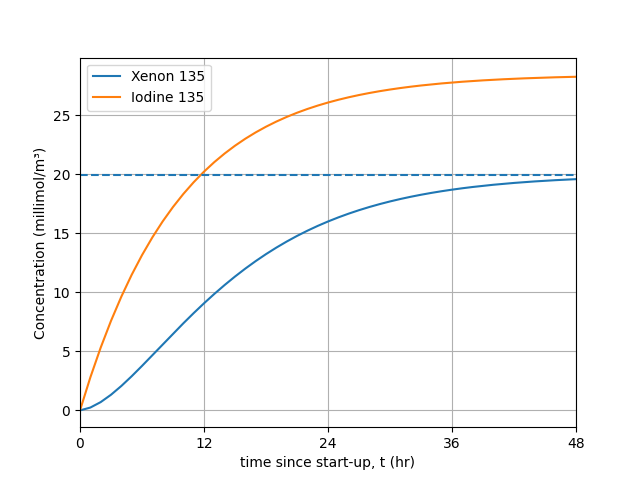
\includegraphics[width=0.99\textwidth]{Xenon/start-up}
                \caption{Concentration of \I and \Xe vs. time following start-up}
            \end{figure}
        \end{column}
        \begin{column}{0.5\textwidth}
            \begin{figure}[ht!]
                \centering
                \includegraphics[width=0.99\textwidth]{Xenon/noHe}
                \caption{Concentration of \I and \Xe vs. time following reactor scram}
            \end{figure}
        \end{column}
    \end{columns}
\end{frame}
\setbeamercolor{background canvas}{bg=Chrome}

\begin{frame}{Xenon Stripper}
    \begin{figure}[ht!]\centering
        \resizebox*{0.95\textwidth}{!}{\begin{tikzpicture}
    \draw[green, very thick] (-2,-0.5) rectangle (2,0.5) ;
    \filldraw[green!10] (-2,-0.5) rectangle (2,0.5);
    \draw node at (0,0) {\small Xenon Stripper};
    %Bottom
    \draw[->,blue] (-1.5,-2)--(-1.5,-0.5);
    \draw node at (-1.35,-1.55) [anchor=west]{\small{$C_{He}^{in} = 0$}};
    \draw node at (-1.65,-1.55) [anchor=east]{\small{$\dot{V}_{He}$}};
    %Top
    \draw[->,blue] (1.5,0.5)--(1.5,2);
    \draw node at (1.65,1.55) [anchor=west]{\small{$C_{He}^{out} = \nicefrac{C_{salt}^{out}}{H^*}$}};
    \draw node at (1.35,1.55) [anchor=east]{\small{$\dot{V}_{He}$}};
    %Left
    \draw[->,red] (-3.75,0)--(-2,0);
    \draw node at (-2.0,0.5) [anchor=east]{\small{$C_{salt}^{in} = Xe(t)$}} ;
    \draw node at (-3.0,-0.5) {\small{$\dot{V}_{salt}$}} ;
    %Right
    \draw[->,red] (2,0)--(5,0);
    \draw node at (2.0,0.5) [anchor = west]{\small{$C_{salt}^{out} = C_{salt}^{in}-C_{He}^{out}\frac{\dot{V}_{He}}{\dot{V}_{salt}}$}};
    \draw node at (3.0,-0.5) [anchor=west]{\small{$\dot{V}_{salt}$}} ;
    \end{tikzpicture}
    
}
         \caption{Schematic Drawing of Xenon Stripping Module}
    \end{figure}
\only<2>{\tiny
    \begin{equation*}\label{eq:diffXe_strip}
        \frac{dXe}{dt} =
        \underbrace{\gamma_{Xe}\Sigma_{f}^{F}{\phi}(t)}_{\text{Fission Yield}}
        +\underbrace{\lambda_{I}I(t)}_{\text{Precursor Decay}}
        -\underbrace{\lambda_{Xe}Xe(t)}_{\text{Beta Decay}}
        -\underbrace{Xe(t)\sigma_{a}^{Xe}{\phi}(t)}_{\text{Radiative Capture}}
        -\underbrace{ \frac{Xe(t)}{\tau_{salt}}\left( H^*\frac{\dot{V}_{salt}}{\dot{V}_{He}}+1 \right)^{-1}}_{\text{Stripping}}
\end{equation*}
}
\end{frame}

\setbeamercolor{background canvas}{bg=White}
\begin{frame}{Xenon Stripping Dynamics}
    \begin{columns}
        \begin{column}{0.5\textwidth}
            \begin{figure}[ht!]
                \centering
                \includegraphics[width=0.99\textwidth]{Xenon/8hr_restart}\caption{Concentration of \I and \Xe vs. time following reactor scram - Restart Mode}
            \end{figure}
        \end{column}
        \begin{column}{0.5\textwidth}
            \begin{figure}[ht!]
                \centering
                \includegraphics[width=0.99\textwidth]{Xenon/standby_restart}
                \caption{Concentration of \I and \Xe vs. time following reactor scram - Standby Mode}
            \end{figure}
        \end{column}
    \end{columns}
\end{frame}
\setbeamercolor{background canvas}{bg=Chrome}
\end{comment}

\end{document}


